% Documento principal del informe de la Entrega 2.
% Copia en el repositorio del proyecto de Overleaf. Única diferencia: aquí el anexo de IA se llama anexo_ia.tex.
% Máximo 10 páginas de cuerpo; la portada y los anexos no cuentan.
% Cada sección vive en su propio .tex para que cada responsable edite la suya.
\documentclass[11pt,a4paper]{article}
\usepackage[utf8]{inputenc}
\usepackage[T1]{fontenc}
\usepackage{lmodern}
\usepackage[spanish]{babel}
\usepackage[margin=2.5cm]{geometry}
\usepackage{graphicx}
\usepackage{booktabs}
\usepackage{array}
\usepackage{longtable}
\usepackage[hidelinks]{hyperref}
\usepackage{xcolor}
\usepackage{soul}
\sethlcolor{yellow}
\usepackage{pdfpages}
\usepackage{amsmath}
\usepackage[font=small,skip=3pt]{caption}
% El cuerpo tiene más de veinte \paragraph; el espacio por defecto antes de cada uno
% (3,25ex) suma casi un cuarto de página. Se aprieta a 1,6ex, que sigue separando bien.
\usepackage{titlesec}
\titlespacing*{\paragraph}{0pt}{1.6ex plus .4ex minus .2ex}{1em}
\setlength{\textfloatsep}{8pt plus 2pt minus 2pt}
\setlength{\intextsep}{8pt plus 2pt minus 2pt}
% figuras/ en Overleaf; ../output/figuras/ al compilar en local desde informe/
\graphicspath{{figuras/}{../output/figuras/}}

% Todas las cifras del informe quedaron verificadas contra output/cifras.md (componente B),
% así que la marca de «por confirmar» está apagada.
\newcommand{\porconfirmar}[1]{#1}

\usepackage{tabularx}

\begin{document}

\begin{titlepage}
  \centering
  {\large IIC3752 Tecnologías para Inteligencia de Negocios\par}
  {\large Escuela de Ingeniería UC - 2026-2\par}
  \vspace{4cm}
  {\LARGE\bfseries Entrega 2\par}
  \vspace{0.5cm}
  {\Large Viña Vallehondo - Grupo 2\par}
  \vspace{3cm}
  {\large Integrantes\par}
  \vspace{0.3cm}
  Diego Da Silva\par
  Nicolás Massa\par
  Sebastián Valdés\par
  Benjamín Suazo\par
  \vfill
  Repositorio: \url{https://github.com/Benjaa7/vina-g2} (etiqueta \texttt{E2}, carpeta \texttt{E2/})\par
  \vspace{0.2cm}
  {\small Prototipo: \url{https://dbc-c40c64f6-aa40.cloud.databricks.com/dashboardsv3/01f1df8721bb10a6b14af51e24530fc6/published?o=7474648132034809}\par}
  \vspace{0.5cm}
  18 de noviembre de 2026
\end{titlepage}

% Sección A · Registro de mejora (máximo 1 página, va primero). Las referencias de sección y página
% se generan con \ref y \pageref: no escribirlas a mano.
\providecommand{\pend}[1]{\textcolor{red}{#1}}
\newcolumntype{L}{>{\raggedright\arraybackslash}X}
\newcolumntype{P}[1]{>{\raggedright\arraybackslash}p{#1}}

\section{Registro de mejora}
\label{sec:mejora}

Este informe es la Entrega~1 corregida, con tres secciones nuevas: arquitectura, prototipo y adopción. La tabla recoge cada observación de la Entrega~1 (E1) y de la Presentación~1 (P1), qué hicimos y dónde quedó el cambio.

\begin{center}
\footnotesize
\renewcommand{\arraystretch}{1.0}
\begin{tabularx}{\textwidth}{@{}r P{0.95cm} L L P{1.35cm}@{}}
\toprule
\# & \textbf{Origen} & \textbf{Observación} & \textbf{Qué hicimos} & \textbf{Dónde} \\
\midrule
1 & E1 &
Cajas y litros es un problema de gobierno de datos; la empresa no declaró el litro como su unidad. &
\textbf{Atendida.} El mandato enuncia la fractura: comercial habla de cajas, operaciones de litros (V). Medir por litro es decisión nuestra (I). El acta lleva una nota de corrección. &
§\ref{sec:mandato}, p.~\pageref{sec:mandato}; acta \\
\addlinespace[2pt]
2 & E1 y P1 &
La definición que mueve el número es la fecha de conversión a pesos, no los 9, 18 o 4,5~L por caja. &
\textbf{Atendida.} Moneda y fecha pasan al cuerpo (USD 11,2\,\%; CLP 10,1\,\% a factura; 6,3\,\% a cobranza) y se eligen en el prototipo. Litros por caja, al anexo~D. &
§\ref{sec:metrica}, p.~\pageref{sec:metrica} \\
\addlinespace[2pt]
3 & E1 y P1 &
Mostrar el 108\,\% sin las líneas corregidas (montos, monedas, botellas). &
\textbf{Atendida.} Con esas líneas sin corregir, el alza sería 17,6\,\% y la mezcla explicaría el 78,2\,\% (M): sigue siendo la causa. Se puede ver en el prototipo. &
§\ref{sec:metrica}, p.~\pageref{tab:sensibilidades} \\
\addlinespace[2pt]
4 & E1 y P1 &
CLP 2.961~MM valoriza el pasado; falta cuánto vale cada punto de gran reserva. &
\textbf{Atendida.} Cada punto de gran reserva en vez de varietal vale CLP 353~MM de margen bruto al año (338 con el dólar de la cobranza). Va en la primera lámina de la P2. &
§\ref{sec:negocio}, p.~\pageref{sec:negocio} \\
\addlinespace[2pt]
5 & E1 &
Las acciones no dicen cuánto cuestan. &
\textbf{Atendida.} Incentivo de CLP 5.000 por caja incremental (CLP 127,1~MM al año para $+2,0$\,pp) y reasignación de stock sin costo; dueño: Gerencia Comercial. &
§\ref{sec:negocio}, p.~\pageref{sec:negocio} \\
\addlinespace[2pt]
6 & P1 &
«Medir y fijar metas» no es una decisión. &
\textbf{Atendida.} Meta de $+2,0$\,pp de Gran Reserva en mercados con recomendación (CLP 706~MM/año de margen), decidida mensualmente por Gerencia Comercial. &
§\ref{sec:negocio}, p.~\pageref{sec:negocio} \\
\addlinespace[2pt]
7 & P1 &
No convertir divisas con un promedio del período. &
\textbf{Atendida.} Toda cifra en pesos se convierte línea por línea con el dólar de su fecha; ya no se usa el 946,34. &
§\ref{sec:negocio}, p.~\pageref{sec:negocio} \\
\addlinespace[2pt]
8 & P1 &
Falta claridad en la fecha de corte y en la unidad de tiempo. &
\textbf{Atendida.} Facturas 1-ene a 31-dic-2025, por semestre; declarado en cada figura, en el prototipo y en la bitácora. &
§\ref{sec:metrica}, p.~\pageref{sec:metrica} \\
\addlinespace[2pt]
9 & P1 &
Explicar el modelo relacional con más detención. &
\textbf{En el informe, sí;} en la P2, no: la única lámina técnica permitida es la arquitectura. &
§\ref{sec:modelo}, p.~\pageref{sec:modelo} \\
\addlinespace[2pt]
10 & E1 &
Profundizar la modularización hacia ETL o ELT. &
\textbf{Atendida.} Arquitectura por capas con sus tres decisiones y pruebas de calidad. &
§\ref{sec:arquitectura}, p.~\pageref{sec:arquitectura} \\
\bottomrule
\end{tabularx}
\end{center}

\vspace{-4pt}
\paragraph{El número, E1 frente a hoy.}

\begin{center}
\footnotesize\setlength{\tabcolsep}{5pt}
\renewcommand{\arraystretch}{1.05}
\begin{tabular}{@{}l r r l@{}}
\toprule
\textbf{Cifra} & \textbf{E1} & \textbf{E2} & \textbf{Cambio} \\
\midrule
Precio medio por litro, 1.\textsuperscript{er} sem. 2025 & 4,574 USD/L & 4,574 USD/L & Ninguno \\
Precio medio por litro, 2.\textsuperscript{o} sem. 2025 & 5,085 USD/L & 5,085 USD/L & Ninguno \\
Alza del precio medio & +11,2\,\% & +11,2\,\% & Ninguno \\
Parte del alza que es mezcla & 108\,\% & 108\,\% & Ninguno \\
Ventas fuera por calidad & 1,6\,\% & 1,6\,\% & Ninguno \\
Valor de la mezcla, CLP & 2.961 MM, venta 2.\textsuperscript{o} sem. & 353 MM/año, margen por punto & Ver nota \\
\bottomrule
\end{tabular}
\end{center}

\noindent La métrica no cambió: ninguna observación tocó su definición ni su universo, y la cadena reproduce las cifras de la E1. Cambia el valor en pesos: ahora es lo que vale cada punto de mezcla hacia adelante (fila~4), en margen y no en venta, y convertido línea por línea con el dólar de su fecha (fila~7).

% Sección · Mandato acordado (de la E1, condensado en la E2 para respetar las 10 páginas).
% Todas las cifras están verificadas contra output/cifras.md (componente B).

\section{Mandato acordado}
\label{sec:mandato}

Cada hallazgo va marcado con su origen: \textbf{(V)} verbalizado por la contraparte, \textbf{(M)} medido por nuestro análisis, \textbf{(I)} inferido por el equipo.

\paragraph{La pregunta.} De las cuatro del README, trabajamos la segunda: el precio promedio por litro que subió, ¿es porque subimos precios o porque vendimos mayor proporción de gran reserva?

\paragraph{Por qué esa.} Sale de la reunión del 4 de septiembre. Sin que se lo preguntáramos, la contraparte dijo que el encargo nace de la conversión entre cajas y litros: «nos dimos cuenta que teníamos un problema y por eso los llamamos» (V). Nombró el vacío que quiere cerrar, «no se disgrega cepa, reserva, gran reserva ni varietal al tomar la decisión» (V), y una fractura de gobierno de datos: «ellos hablan de cajas, nosotros hablamos de litros» (V), porque comercial vende cajas y operaciones produce litros. Medir por litro es decisión nuestra, no una instrucción del cliente: es la única unidad que compara precios entre formatos de caja (I). El dato confirma que la pregunta no es obvia: el precio medio por litro de exportación subió 11,2\,\% entre semestres de 2025, de 4,574 a 5,085 USD/L, mientras los precios de lista bajaron entre 0,15\,\% y 0,19\,\% en los tres tiers y la gran reserva pasó de 22,7\,\% a 32,5\,\% de los litros (M).

\paragraph{Por qué no las otras.} La primera, el tipo de cambio, queda como contexto: la contraparte no lo planteó como problema y declaró no tener política formal para valorizar exportaciones (V). La tercera, margen por mercado, no se puede responder con lo entregado: faltan aranceles, costos de despacho y el tramo de dólar a euro de los clientes europeos (V). La cuarta, con qué fecha convertir a pesos, no es otra pregunta sino una decisión de definición de la nuestra, y la tratamos en la sección~\ref{sec:metrica}.

\paragraph{El hilo de correo y la definición que quedó abierta.} El hilo se abrió el 8 de septiembre con el acta. Las consultas enviadas por esa vía no fueron respondidas, así que la equivalencia de caja a litro, el tratamiento del monto neto y la estacionalidad del alza quedan como supuestos cuantificados en la bitácora (S1, S3 y S8). La equivalencia era la definición abierta: operaciones afirmó que «no todas las cajas tienen el mismo número de litros» (V), pero el maestro de costos declara 9,0 litros para los dos formatos, 12$\times$750 y 6$\times$1500 (M), y el precio de lista por caja del magnum, USD 77,26, coincide con el del gran reserva estándar, USD 77,20 (M), lo que solo se sostiene si ambos rinden los mismos litros (I). La cerramos en 9,0 litros: cuando el cliente y el dato no coinciden, adoptamos el dato si otra fuente lo verifica, y aquí la verificación viene de otro archivo. Con 18 o 4,5 litros por caja magnum la mezcla sigue explicando el 108\,\% del alza (anexo~D).

% Sección B · Arquitectura y operación de la cadena (componente B, 25 %). Reemplaza a la «Cadena ejecutable» de la E1.
% Requiere en el preámbulo: graphicx, booktabs, array, xcolor. Las cifras salen de E2/output/cifras.md y dq_resultados.csv.
\providecommand{\pend}[1]{\textcolor{red}{#1}}

\section{Arquitectura y operación de la cadena}
\label{sec:arquitectura}

La cadena de la E1 corría en un computador. Ahora corre en Databricks Free Edition como un job de ocho pasos, con las tablas en Unity Catalog, pruebas de calidad antes de publicar y un tablero que lee el resultado (figura~\ref{fig:arquitectura}).

\paragraph{Cómo se corre de cero.} En un workspace de Free Edition se crea una carpeta Git con el repositorio (\emph{Workspace $\rightarrow$ Create $\rightarrow$ Git folder}) y se ejecuta \emph{Run all} en \texttt{E2/correr\_e2}. Ese notebook crea el job \texttt{vallehondo\_e2}, lo ejecuta, muestra las pruebas y las cifras y publica el tablero, sin instalar nada ni configurar credenciales: las fuentes van en el repositorio. Demora unos 6 minutos. Sobre un catálogo vacío reprodujo byte a byte el registro de limpieza de la E1. El 17 de noviembre la corrimos en un workspace nuevo, de otra cuenta, siguiendo solo el README: 8 de 8 pasos terminaron bien, pasaron las 15 pruebas y salieron las mismas cifras del informe. Tardó unos 14 minutos, 6 de ellos esperando el primer cómputo de la cuenta nueva; la API del dólar no respondió y la cadena usó el respaldo. La ventana para crear la carpeta Git quedó cargando, así que la creamos con la misma URL desde la API; el README lo explica.

\begin{figure}[!htbp]
  \centering
  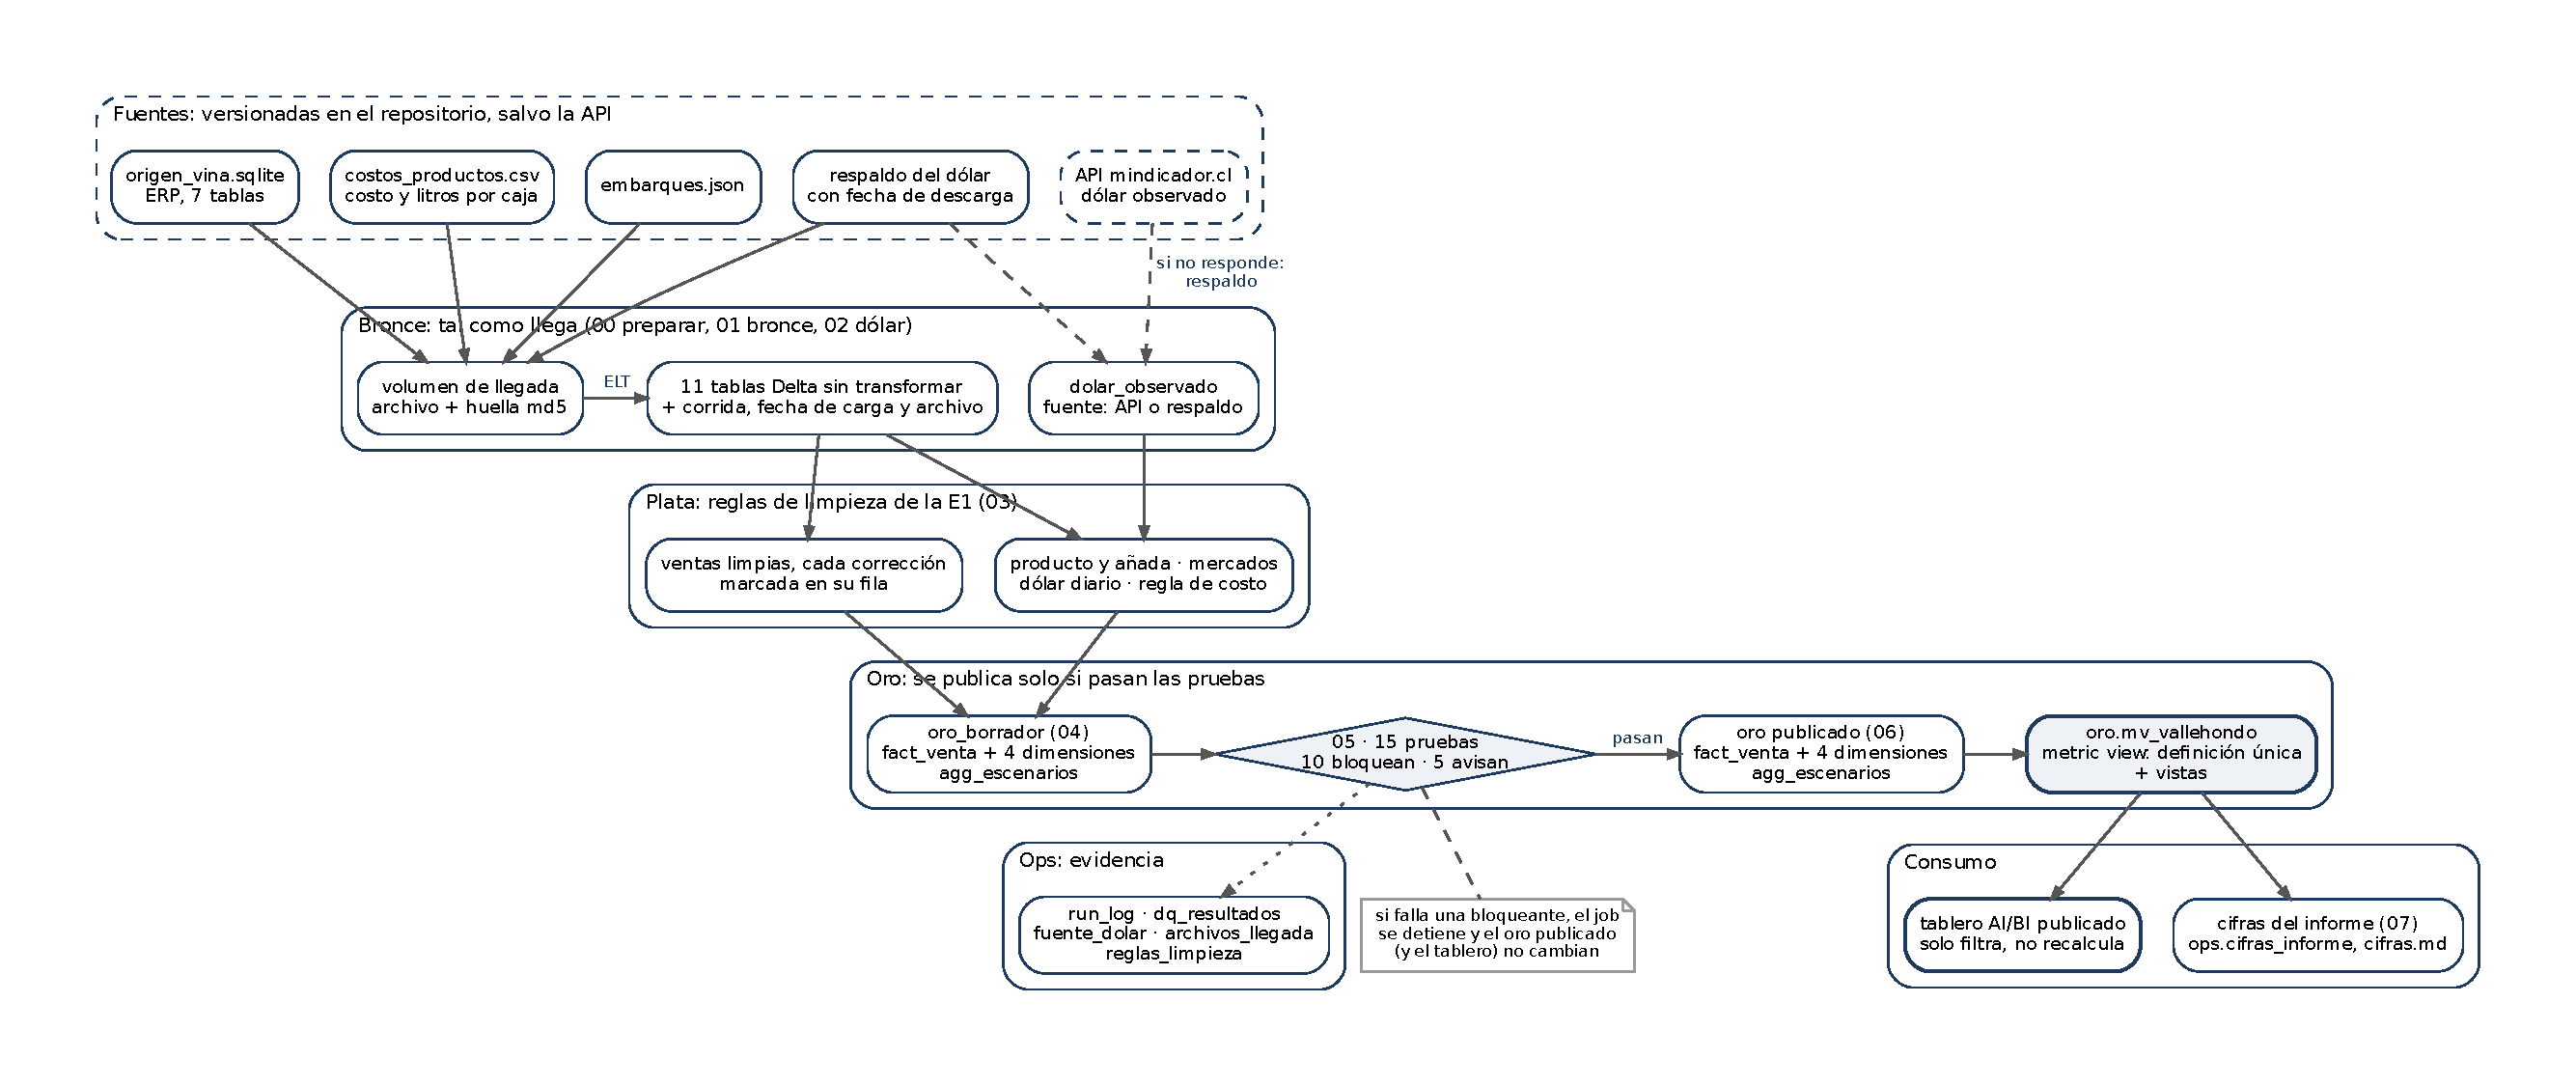
\includegraphics[width=0.82\textwidth]{arquitectura.pdf}
  \caption{Arquitectura por capas. Los números entre paréntesis son los pasos del job. Fuente: elaboración propia.}
  \label{fig:arquitectura}
\end{figure}

\paragraph{Qué hace cada capa.} \textbf{Bronce} guarda las cuatro fuentes tal como llegan, como tablas Delta, con la corrida, la fecha de carga y el archivo de origen. \textbf{Plata} aplica las reglas de limpieza de la E1 (anexo~B); cada corrección queda marcada en su fila, y eso permite apagarla. \textbf{Oro} tiene el modelo de la sección~\ref{sec:modelo}, la tabla de escenarios y la definición única de la métrica; se arma en un esquema borrador y se publica solo si las pruebas lo permiten. \textbf{Ops} guarda la evidencia de cada corrida: pasos, pruebas y origen del dólar. El \textbf{tablero} solo filtra; no recalcula nada.

\paragraph{Tres decisiones.}
\begin{itemize}\setlength\itemsep{1pt}
\item \textbf{ELT y no ETL.} Las fuentes entran crudas a bronce y se transforman dentro de Databricks. Si cambia una regla, como los litros por caja, se reprocesa desde bronce sin volver a extraer, y el linaje queda en una sola plataforma. El costo: depender de la cuota diaria de cómputo de Free Edition.
\item \textbf{Carga completa en cada corrida.} Todas las tablas se reemplazan, nunca se agregan: con 13.845 líneas la corrida dura minutos, y agregar sobre lo anterior duplicaría ventas si un paso se reintenta. Una prueba compara cada corrida con el oro publicado: dos corridas dejan 13.845 líneas y USD 73.435.428,61.
\item \textbf{Si la API del dólar falla, respaldo con fecha; si no hay respaldo, no se publica.} Desde Databricks, mindicador.cl responde a veces: en la corrida oficial respondió para 2025 y no para 2026 (M). Cuando falla, la cadena usa el respaldo versionado en el repositorio (descargado el 2 y el 12 de octubre de 2026), lo registra, y el pie del tablero muestra la fuente y su fecha. Si ninguno cubre una fecha, la prueba del dólar bloquea y el tablero sigue mostrando la última corrida buena.
\end{itemize}

\paragraph{Pruebas de calidad.} Quince pruebas corren en cada ejecución, entre el oro borrador y su publicación. Diez \emph{bloquean} el job si fallan: una por fuente (ERP, JSON, CSV y dólar) y las que protegen la métrica (clave única del hecho, sin huérfanos, fechas dentro del período, conciliación entre plata y oro). Cinco \emph{avisan}: rangos de precio y descuento, cifras de control de la E1, idempotencia y los dos pisos del acuerdo de servicio. El anexo~B detalla qué verifica cada una, qué hace si falla y su resultado en la última corrida.

\paragraph{Linaje.} Unity Catalog dibuja solo el linaje entre tablas. La figura~\ref{fig:linaje} lo completa hasta la pantalla para cada campo de la métrica: de qué columna sale, qué regla lo corrige, en qué campo del hecho queda y dónde se ve. El ingreso, por ejemplo, nace en el precio, el descuento, el monto y la moneda de la venta; pasa por los 555 montos recalculados y las 542 monedas imputadas; queda en \texttt{monto\_neto\_usd} y llega al tablero como numerador de \texttt{precio\_por\_litro}.

\begin{figure}[!htbp]
  \centering
  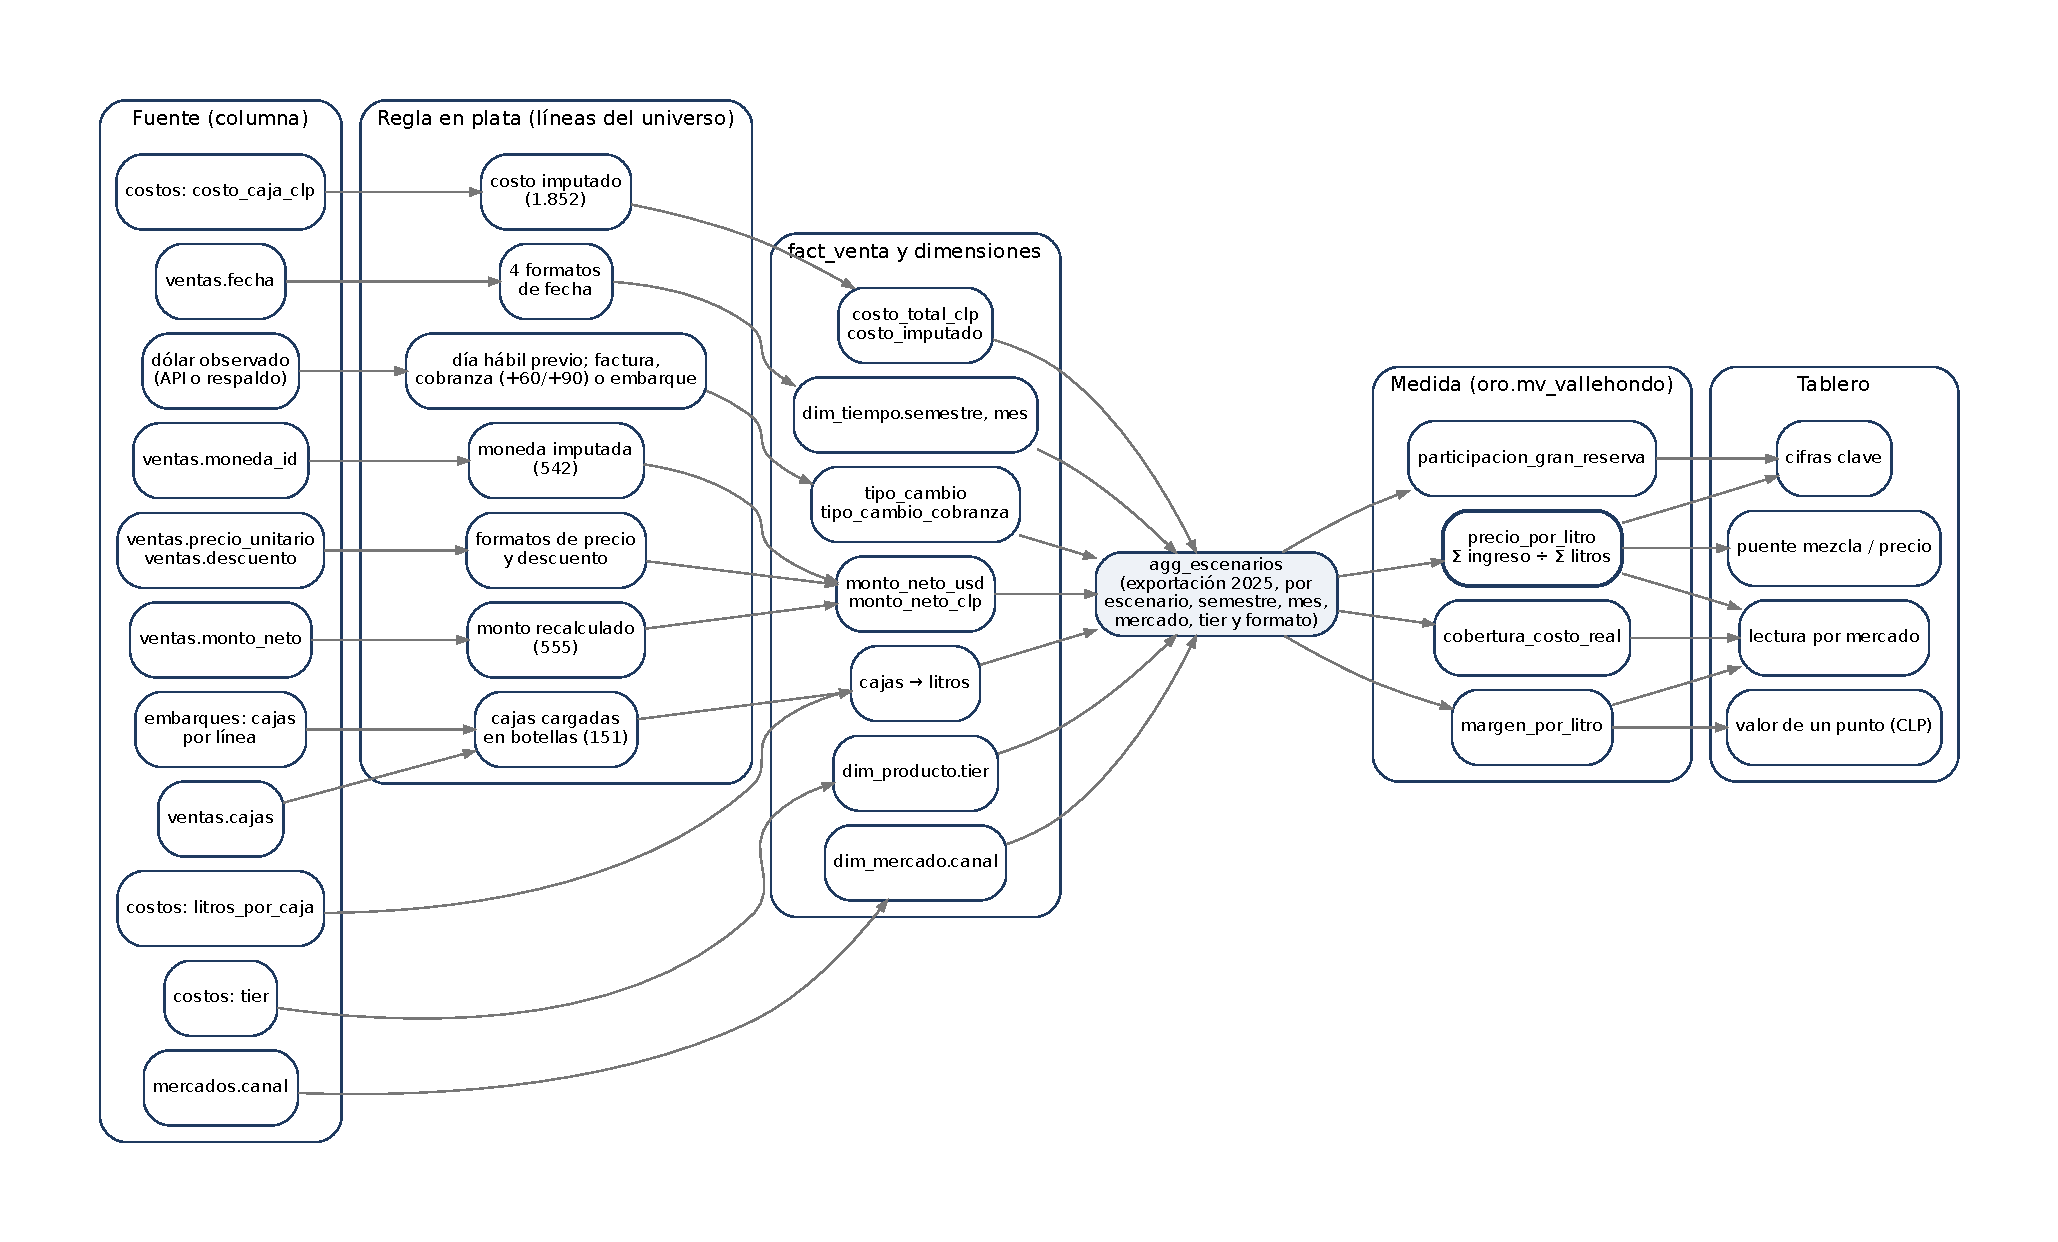
\includegraphics[width=0.56\textwidth]{linaje.pdf}
  \caption{Linaje de la métrica, de la columna de origen a la pantalla. Fuente: elaboración propia a partir del código de la cadena.}
  \label{fig:linaje}
\end{figure}

\paragraph{Acuerdo de servicio de \texttt{fact\_venta}.} Los dos pisos de completitud se miden en cada corrida como pruebas que avisan, y la frescura con la fecha de la última corrida; el pie del tablero muestra las tres cosas.

\begin{center}\footnotesize
\renewcommand{\arraystretch}{1.15}
\begin{tabular}{@{}l p{5.6cm} p{6.4cm}@{}}
\toprule
\textbf{Compromiso} & \textbf{Valor} & \textbf{Por qué ese umbral} \\
\midrule
Frescura & Mensual, a más tardar 5 días hábiles después del cierre & Comercial arma hoy la cifra una vez al mes (V) \\
Completitud & Al menos 98\,\% de las ventas registradas llega a \texttt{fact\_venta}; al menos 80\,\% de los litros con costo real & Hoy llegan 99,0\,\% y hay 82,8\,\% con costo real; bajo esos pisos el margen deja de ser defendible (M) \\
Calidad & 100\,\% de las pruebas que bloquean y al menos 90\,\% del total en verde & Una prueba que bloquea en rojo es un número que no se puede defender \\
Dueño & Departamento Comercial & Es quien hoy descarga el ERP y arma la cifra mensual (V) \\
\bottomrule
\end{tabular}
\end{center}


% Sección C · Modelo dimensional y una sola definición (componente C, 10 %). Reemplaza al «Modelo dimensional» de la E1.
% Requiere en el preámbulo: graphicx, booktabs, array. Las cifras salen de E2/output/cifras.md.

\section{Modelo dimensional y una sola definición}
\label{sec:modelo}

Modelamos un solo proceso de negocio, la venta: cada vez que se factura una línea de vino. Es una tabla de hechos transaccional con cuatro dimensiones a un salto (figura~\ref{fig:modelo}); la fuente viene normalizada en tablas encadenadas (ventas, mercados, zonas) y la aplanamos en una estrella porque país y zona son niveles de una misma jerarquía.

\begin{quote}
\textbf{Grano.} Una fila de \texttt{fact\_venta} es una línea de venta facturada: un producto de una añada, vendido a un cliente en una fecha.
\end{quote}

\begin{figure}[!htbp]
  \centering
  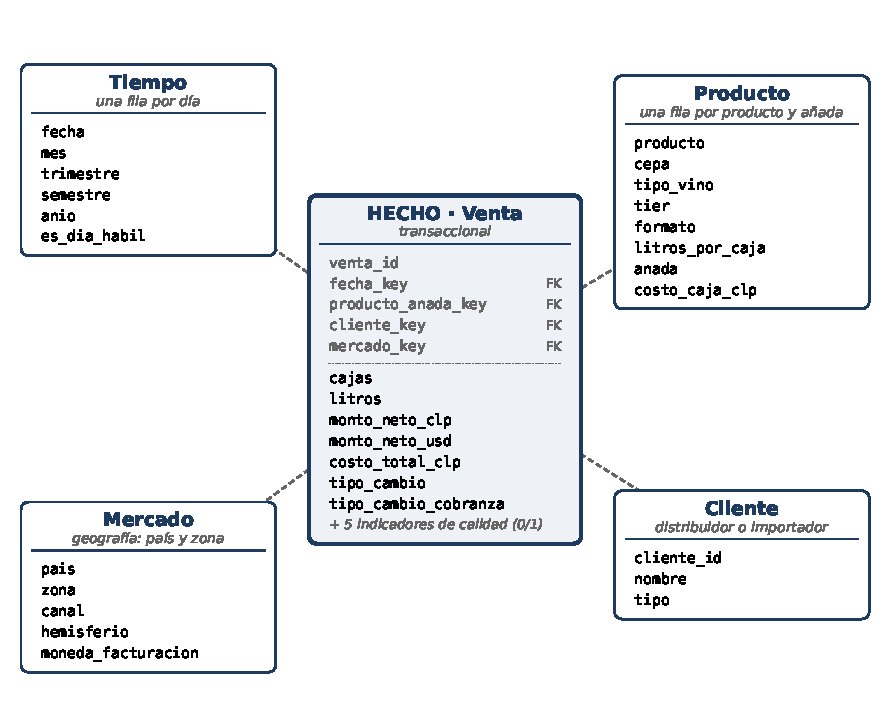
\includegraphics[width=0.47\textwidth]{modelo_estrella.pdf}
  \caption{Modelo estrella de la venta. Diccionario de datos, con la unidad de cada campo, en el anexo~C. Fuente: elaboración propia.}
  \label{fig:modelo}
\end{figure}

\paragraph{Por qué este grano.} No hay en la fuente un nivel más fino, y uno más grueso destruye la pregunta: para separar precio de mezcla, cada fila debe conservar su tier y sus litros. Por lo mismo, el hecho guarda solo lo que se suma (cajas, litros, montos en pesos y en dólares, costo) y nunca el precio por litro: una razón de sumas no es aditiva y se calcula en cada corte. De las 13.845 filas, 10.672 son exportaciones facturadas en 2025 y forman el universo de la métrica.

\paragraph{Las dimensiones.} \texttt{dim\_producto} tiene una fila por producto y añada (96), porque el costo por caja depende de la añada; ahí viven el tier y \texttt{litros\_por\_caja}. \texttt{dim\_mercado} trae el canal y el hemisferio, que fija los días de cobranza, y \texttt{dim\_tiempo} el semestre y si el día tuvo dólar publicado. Quedan fuera el embarque, otro proceso con su propio grano que solo corrige las cajas cargadas en botellas, el vendedor, redundante con la zona, y el flete y los aranceles, que no están en ninguna fuente.

\paragraph{Qué cambió respecto de la E1, y por qué.} El grano y las dimensiones no cambiaron: ninguna observación los cuestionó, y la de la P1 pedía explicarlos con más detención, no rehacerlos. Al hecho se le agregaron cinco columnas para que cada escenario de la sección~\ref{sec:metrica} salga de la misma tabla y no de una segunda cadena: el dólar a la fecha estimada de cobranza y a la de embarque, la marca de costo imputado, y las cajas y el monto tal como venían en el ERP. Con las marcas que ya tenía (monto recalculado, cajas corregidas, moneda imputada), la métrica se puede recalcular con cualquier corrección apagada.

\paragraph{La métrica, definida una sola vez.} Las fórmulas viven en un solo objeto del oro: la \emph{metric view} \texttt{oro.mv\_vallehondo} de Unity Catalog, que es la capa semántica de la cadena (tabla~\ref{tab:medidas}). Lee de \texttt{agg\_escenarios}, que guarda solo sumas de \texttt{fact\_venta} por semestre, mes, mercado, tier y formato para cada uno de los 60 escenarios (4 monedas y fechas del dólar, 3 equivalencias de litros por caja y 5 combinaciones de correcciones); las razones se calculan al consultar.

\begin{table}[!htbp]
\centering\small
\caption{Medidas de la definición única (\texttt{oro.mv\_vallehondo}).}
\label{tab:medidas}
\begin{tabular}{@{}l l l@{}}
\toprule
\textbf{Medida} & \textbf{Fórmula} & \textbf{Unidad} \\
\midrule
\texttt{precio\_por\_litro} & $\sum$ ingreso neto $\div$ $\sum$ litros & USD/L o CLP/L \\
\texttt{margen\_por\_litro} & $\sum$ (ingreso neto $-$ costo de producto) $\div$ $\sum$ litros & CLP/L \\
\texttt{participacion\_gran\_reserva} & litros de gran reserva $\div$ litros & \% \\
\texttt{cobertura\_costo\_real} & litros con costo no imputado $\div$ litros & \% \\
\bottomrule
\end{tabular}
\end{table}

\noindent El tablero, las vistas de la descomposición y el paso que escribe las cifras del informe consultan estas medidas; no hay una segunda fórmula en Python ni en el tablero. Por eso el precio medio por litro tiene el mismo nombre y el mismo número en el informe, en \texttt{cifras.md} y en la pantalla: 4,574 y 5,085 USD/L, +11,2\,\%. Las definiciones alternativas de la E1, los litros por caja de 18 o 4,5 y la conversión a pesos con otra fecha, siguen disponibles como filtros del prototipo: la contraparte las ve sin que recalculemos nada.

% Sección D · Métrica y sensibilidad.
% El desarrollo (datos de entrada, cálculo tier por tier, métodos alternativos y
% las otras tres decisiones) está en el anexo D, para respetar el límite de 6 páginas.

\section{Métrica y sensibilidad}
\label{sec:metrica}

\paragraph{Qué medimos.} La métrica es el precio medio por litro de exportación de cada semestre de 2025:
\[
P = \frac{\sum_i M_i}{\sum_i L_i}, \qquad L_i = C_i \times k_i,
\]
donde, para cada línea de venta $i$, $M_i$ es el monto neto en USD (después de descuento), $L_i$ son los litros vendidos, $C_i$ son las cajas y $k_i$ son los litros por caja de su producto. La suma recorre las líneas de \texttt{fact\_venta} del canal exportación con fecha de factura en el semestre (10.672 en el año), incluidas las de merma, con signo negativo. Es una razón de sumas, no un promedio de precios. Entre el 1.\textsuperscript{er} y el 2.\textsuperscript{o} semestre, $P$ subió de 4,574 a 5,085 USD/L: +0,511 USD/L, un 11,2\,\%.

\paragraph{Por qué no basta con mirar $P$.} Un precio medio puede subir por dos razones distintas: porque cada vino se vende más caro (\emph{efecto precio}) o porque, con los mismos precios, se vende una mayor proporción del vino caro (\emph{efecto mezcla}). Para separarlas usamos la descomposición estándar precio-mezcla (Kitagawa, 1955; Horngren, Datar y Rajan, \emph{Cost Accounting}): para cada tier $t$, con $w_t$ su proporción de los litros y $p_t$ su precio por litro, el cambio de $P$ se reparte en tres términos que suman exactamente el alza: mezcla $\sum_t (w_{t,2}-w_{t,1})\,p_{t,1}$, precio $\sum_t w_{t,1}\,(p_{t,2}-p_{t,1})$ y cruzado $\sum_t (w_{t,2}-w_{t,1})(p_{t,2}-p_{t,1})$. El cálculo tier por tier está en el anexo~D. El criterio, fijado antes de mirar los resultados: el alza es de mezcla si ese efecto explica más de la mitad del cambio con todos los métodos y definiciones alternativas. No usamos pruebas de significancia: los datos son todas las ventas del año, no una muestra, y la incertidumbre viene de nuestras definiciones, que es lo que miden las sensibilidades.

\paragraph{Resultado.}

\begin{center}
\small
\begin{tabular}{l r r}
\hline
\textbf{Efecto} & \textbf{USD/L} & \textbf{\% del alza} \\
\hline
Mezcla & +0,551 & +108\,\% \\
Precio & $-$0,035 & $-$7\,\% \\
Cruzado & $-$0,005 & $-$1\,\% \\
\hline
\textbf{Cambio total} & \textbf{+0,511} & \textbf{100\,\%} \\
\hline
\end{tabular}
\end{center}

\noindent Vender 9,8 puntos más de gran reserva, el tier más caro, suma 0,81 USD/L al precio medio; vender 9,3 puntos menos de varietal resta 0,23. El efecto precio es negativo en los tres tiers: los precios de lista bajaron entre 0,15\,\% y 0,19\,\% y el descuento medio subió de 3,82\,\% a 4,40\,\% (ponderados por cajas). El cruzado es el 1\,\% del alza, así que la repartición no es ambigua. Según el criterio fijado, \textbf{el alza es de mezcla}.

\paragraph{La decisión de definición: moneda y fecha de conversión.}\label{par:fecha_dolar} La viña vende en dólares (V), pero sus costos y su caja están en pesos, y finanzas mira el resultado en pesos. Convertir exige elegir con qué dólar: el del día de la factura o el del día en que se cobra (factura más 60 días en el hemisferio sur y 90 en el norte, según la contraparte (V)). Cada línea se convierte con el dólar observado de su propia fecha, nunca con un promedio del período. Esta decisión sí mueve el número:

\begin{center}
\small
\renewcommand{\arraystretch}{1.15}
\begin{tabular}{@{}l r@{}}
\toprule
\textbf{Definición} & \textbf{Alza del precio medio por litro} \\
\midrule
USD (adoptada) & +11,2\,\% \\
CLP, dólar de la fecha de factura & +10,1\,\% \\
CLP, dólar de la fecha de cobranza & +6,3\,\% \\
\bottomrule
\end{tabular}
\end{center}

\noindent Según la fecha que se elija, el alza en pesos va de 10,1\,\% a 6,3\,\%: casi la mitad del 11,2\,\% en dólares. La diferencia es el dólar, que bajó entre semestres: los mismos dólares se convirtieron en menos pesos, y con la fecha de cobranza la caída es mayor porque el dólar se toma aún más tarde (M). Descartamos la fecha de embarque: el 30\,\% de las líneas de embarque tiene fecha anterior a la factura (M).

\paragraph{Qué cambia, qué no y por qué nos quedamos con dólares.} Cambia el tamaño del alza en pesos, no su causa: la caída del dólar no es ni precio ni mezcla, solo le resta al alza (I). Medimos en dólares porque los contratos se firman en esa moneda (V) y así la mezcla queda separada del tipo de cambio. La versión en pesos, la que llega a caja y mira finanzas, se elige en el prototipo.

\paragraph{Las demás decisiones no cambian la conclusión.} Para cada una repetimos el análisis con la opción que no elegimos:

\begin{center}
\small
\renewcommand{\arraystretch}{1.15}
\begin{tabular}{@{}l l l r@{}}
\toprule
\textbf{Decisión} & \textbf{Adoptada} & \textbf{Alternativa} & \textbf{Mezcla, \% del alza} \\
\midrule
Litros por caja magnum & 9,0 L (maestro de costos) & 18 o 4,5 L & 108,2\,\% \\
Correcciones de limpieza & Aplicadas & Sin aplicar (ERP) & 78,2\,\% \\
\bottomrule
\end{tabular}
\label{tab:sensibilidades}
\end{center}

\noindent Con la definición adoptada, la mezcla explica el 107,9\,\% del alza, y en ambas alternativas supera el 50\,\% del criterio. Sin aplicar las correcciones baja a 78,2\,\%: las cajas cargadas en botellas y los montos mal registrados meten ruido en el precio por litro, pero aun así la mezcla explica la mayor parte del alza. Las alternativas de 18 y 4,5\,L por caja son extremos hipotéticos que no cambian la respuesta; su detalle y las demás sensibilidades de la Entrega~1 (método de descomposición, merma y precio de lista) están en el anexo~D.
% Sección nueva · Prototipo (componente D, 25 %). Tablero: Benja. Prueba de uso: quien la aplicó.
% Requiere en el preámbulo: graphicx, booktabs, xcolor, hyperref. Lo marcado con \pend{...} sale en rojo.
\providecommand{\pend}[1]{\textcolor{red}{#1}}

\section{Prototipo}
\label{sec:prototipo}

El prototipo es un tablero de Databricks (AI/BI) que responde la pregunta en una pantalla. Lee directo del oro de la cadena y se vuelve a publicar cada vez que la cadena corre: no tiene datos pegados a mano.\footnote{\url{https://dbc-c40c64f6-aa40.cloud.databricks.com/dashboardsv3/01f1df8721bb10a6b14af51e24530fc6/published?o=7474648132034809}. El ayudante y el profesor tienen acceso al workspace.}

\paragraph{Para quién y cada cuánto.} Para la gerencia comercial y operaciones, una vez al mes, después del cierre: en esa reunión se fija y se revisa la meta de participación de gran reserva por mercado (sección~\ref{sec:negocio}). Reemplaza la planilla que comercial arma hoy descargando el ERP a Excel (V).

\paragraph{Una pregunta en una pantalla.} La primera página sigue la anatomía de la clase~7 (figura~\ref{fig:tablero}). El título es la pregunta; debajo, el período y los filtros (moneda y fecha del dólar, correcciones, litros por caja y mercado), cada uno siempre con un valor, para que una cifra nunca mezcle escenarios. Arriba a la izquierda va la \textbf{cifra clave} con su comparación: el precio por litro subió 11,2\,\% (de 4,574 a 5,085 USD/L), la mezcla explica el 108\,\% del alza y la gran reserva pasó de 22,7\,\% a 32,5\,\% de los litros. Al lado, el \textbf{valor para decidir}: un punto de gran reserva en vez de varietal vale CLP 353 millones de margen bruto al año (338 con el dólar de la cobranza). Debajo, el \textbf{gráfico que explica la cifra}: lo que aportan mezcla, precio y cruzado junto al alza total, y la participación y el precio por litro de cada tier. Al final, el \textbf{corte por mercado} en tabla y el \textbf{pie}: última actualización, pruebas en verde, origen y fecha del dólar, período y dueño del dato.

\begin{figure}[!htbp]
  \centering
  \IfFileExists{figuras/tablero.png}%
    {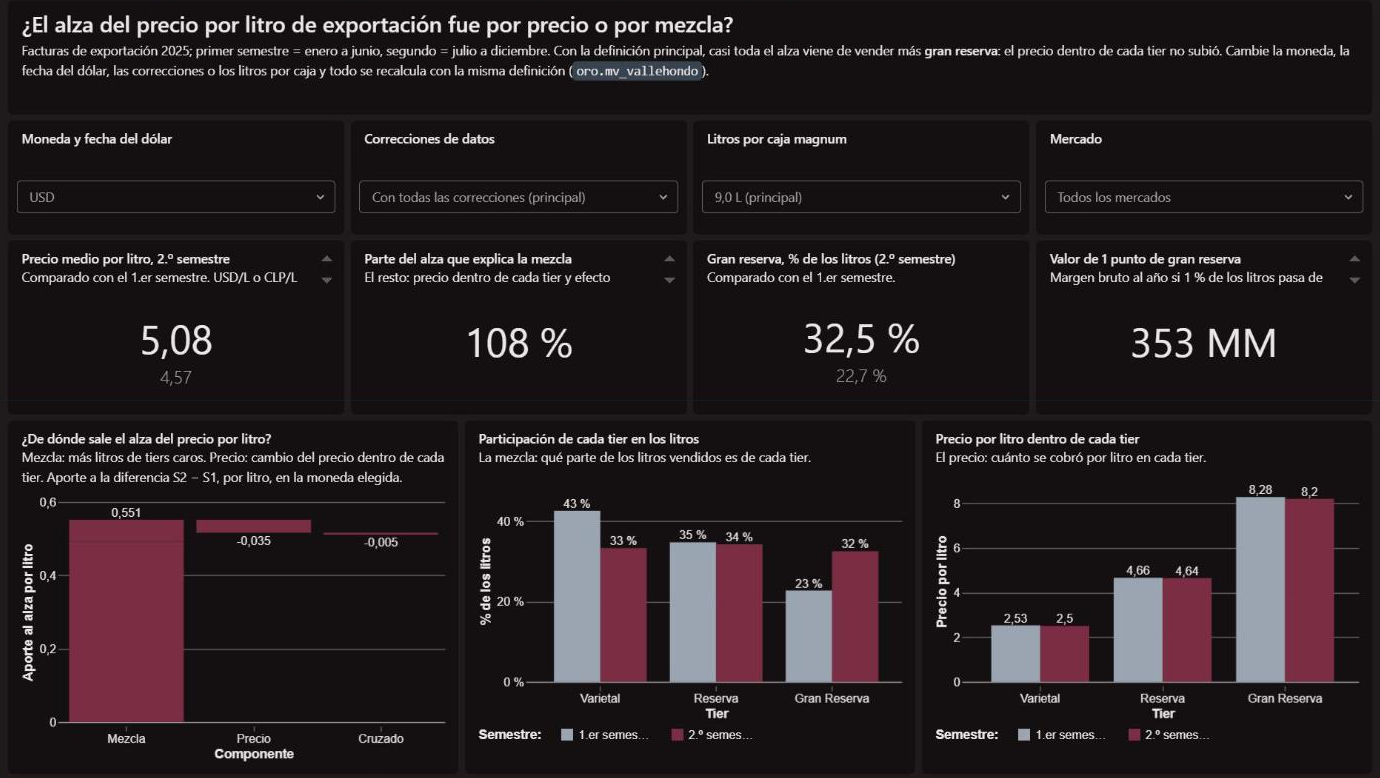
\includegraphics[width=0.66\textwidth]{tablero.png}}%
    {\fbox{\parbox[c][3.5cm][c]{0.9\textwidth}{\centering\pend{Captura de la parte superior de la página «Respuesta» (filtros, cifras clave y gráficos), subida como figuras/tablero.png}}}}
  \caption{Página «Respuesta» del tablero, con la definición principal. Fuente: tablero AI/BI de Databricks sobre el oro de la cadena.}
  \label{fig:tablero}
\end{figure}

\paragraph{Recomendación o hipótesis, con la regla escrita.} Un mercado es \emph{recomendación} si repite el patrón del total con datos suficientes: su precio por litro sube, la mezcla explica al menos el 80\,\% del alza, la gran reserva gana al menos 5 puntos, al menos el 80\,\% de sus litros tiene costo real y tiene al menos 300 líneas; si falla una condición es \emph{hipótesis}, y el tablero dice cuál. Con la definición principal los 10 mercados son recomendación, con la mezcla entre el 97\,\% y el 104\,\% del alza (M). Brasil, el único del hemisferio sur, también, con la gran reserva de 22,7\,\% a 31,5\,\%: el cambio no parece efecto de la temporada navideña del norte (I). Sin las correcciones, México pasa a hipótesis: la mezcla explicaría solo el 49\,\% de su alza.

\paragraph{La segunda página es la de la definición.} Abre con la decisión que más mueve el número: una tabla pone lado a lado el precio por litro, el alza y la parte de la mezcla en USD y con cada fecha del dólar. Debajo están el precio por tier y la gran reserva mes a mes, leídos de la definición única, las fórmulas y las 15 pruebas de la última corrida. El tablero solo filtra: con la definición principal, sus cifras son las de \texttt{cifras.md} y las de este informe.

\paragraph{Prueba de uso.} La hicieron por separado y sin ayuda Italo Suazo e Ignacio Quinteros, ingenieros que usan Power BI y son ajenos al grupo y al curso, con tres preguntas: (1)~cuánto subió el precio por litro y qué parte es mezcla; (2)~cuánto sube en pesos con el dólar de la cobranza; (3)~cuánto vale un punto de gran reserva y si Brasil es recomendación o hipótesis. Trabajaron sobre una captura de la página «Respuesta», así que no podían cambiar filtros ni bajar a la tabla de mercados. El detalle, con lo que le costó a cada uno, está en el anexo~E.

\begin{center}\footnotesize
\renewcommand{\arraystretch}{1.05}
\begin{tabular}{@{}l c c >{\raggedright\arraybackslash}p{4.4cm} >{\raggedright\arraybackslash}p{5.2cm}@{}}
\toprule
\textbf{Persona} & \textbf{Preg.} & \textbf{Tiempo} & \textbf{¿Respondió?} & \textbf{Qué cambiamos} \\
\midrule
Italo Suazo & 1 & 3 min & Sí; calculó el 11,2\,\% a mano & Cifra nueva con el alza en porcentaje \\
 & 2 & 2 min & No: dijo que con la pantalla no se podía saber & Tabla de monedas y fechas del dólar en la página 2 \\
 & 3 & 4 min & En parte: 353 MM, leídos como USD; no vio Brasil & «MM CLP» en el título del valor \\
\midrule
Ignacio Quinteros & 1 & 2 min & Sí: 11\,\% y 108\,\% & Barra del alza total en vez de la cascada \\
 & 2 & 1 min & No: había que cambiar el filtro & La misma tabla de la página 2 \\
 & 3 & 3 min & En parte: 353 MM («supongo CLP»); no vio Brasil & Textos y leyendas sin cortes \\
\bottomrule
\end{tabular}
\end{center}

\noindent La pregunta 2 tampoco se respondía con el tablero vivo sin cambiar un filtro y calcular a mano; ahora se lee en la tabla de la página 2: con el dólar de la cobranza el precio por litro en pesos sube 6,3\,\%, contra 10,1\,\% con el de la factura.

\paragraph{Lista de verificación de la clase 7.} (1) \emph{Qué pregunta responde}: si el alza del precio por litro fue por precio o por mezcla, y cuánto vale mover la mezcla. (2) \emph{Para quién y cada cuánto}: gerencia comercial y operaciones, una vez al mes. (3) \emph{Dónde está la cifra clave}: arriba a la izquierda, con su comparación contra el semestre anterior. (4) \emph{Si cada gráfico calza con su pregunta}: el del alza separa mezcla de precio, las barras por tier muestran qué tier se movió y la tabla dice en qué mercados se repite. (5) \emph{Ejes truncados y totales}: ningún eje está truncado; el gráfico del alza parte de cero y muestra el total que suman mezcla, precio y cruzado. (6) \emph{Quién certificó las definiciones del pie}: la cadena, con 15 de 15 pruebas en verde, la fuente y la fecha del dólar; el dueño del dato es el Departamento Comercial.

% Sección E · Caso de negocio, recomendación y plan de adopción (15 %). Extensión: 2 páginas.

\section{Caso de negocio, recomendación y plan de adopción}
\label{sec:negocio}

\paragraph{Contexto histórico frente a valor accionable.}
En la Entrega~1 se estimó que el cambio de mezcla ocurrido en el segundo semestre de 2025 equivalió a CLP~2.961~millones en ingreso de exportación (CLP~1.664~millones medidos en margen bruto de producto). Sin embargo, esa cifra describe un resultado pasado y no constituye una decisión operativa. Para habilitar una decisión gerencial, valorizamos cada punto porcentual de mezcla futura en \textbf{pesos de margen bruto de producto} (ingreso neto menos costo de producto, sin incluir flete internacional ni aranceles; supuesto~S16), sobre el volumen anual de exportación de 2025 (11,44~millones de litros; 1,27~millones de cajas de 9,0\,L):
\begin{itemize}\setlength\itemsep{2pt}
  \item \textbf{Sustitución de Varietal por Gran Reserva:} Cada punto porcentual adicional de Gran Reserva en reemplazo de Varietal (márgenes unitarios de 3.997 y 911\,CLP/L, respectivamente) genera \textbf{CLP~353~millones} de margen bruto adicional al año con tipo de cambio a fecha de factura, equivalente a \textbf{CLP~27.766 por cada caja} desplazada (12.709 cajas por punto).
  \item \textbf{Sustitución de Reserva por Gran Reserva:} Si el desplazamiento proviene de Reserva (margen de 2.092\,CLP/L), cada punto aporta \textbf{CLP~218~millones} anuales (CLP~17.145 por caja).
  \item \textbf{Sensibilidad cambiaria:} Al convertir con fecha estimada de cobranza ($+60$ días hemisferio sur, $+90$ norte), el valor por punto pasa de CLP~353~millones a \textbf{CLP~338~millones} al año (CLP~26.566 por caja). La caída de 4,2\,\% no altera la conveniencia económica de la decisión.
\end{itemize}

\paragraph{Recomendación accionable, costo y punto de equilibrio.}
\begin{quote}
\textbf{Decisión recomendada:} Fijar una meta comercial de incrementar en \textbf{+2,0 puntos porcentuales} la participación de Gran Reserva sobre los litros totales de exportación para 2026 (pasando del 32,5\,\% registrado en el segundo semestre de 2025 al 34,5\,\%) en reemplazo de Varietal, focalizada en los mercados clasificados como \emph{recomendación} por el tablero. Esta meta genera un retorno esperado de \textbf{CLP~706~millones} de margen bruto anual (CLP~676~millones a fecha de cobranza), con un costo estimado de \textbf{CLP~127,1~millones} al año, y es decidida y monitoreada mensualmente por la \textbf{Gerencia Comercial} utilizando el tablero de Databricks.
\end{quote}

\noindent Para alcanzar los $+2,0$\,pp (25.418 cajas incrementales de Gran Reserva), se evalúan dos palancas operativas bajo el supuesto de volumen total y márgenes unitarios constantes (S15 y S18):
\begin{enumerate}\setlength\itemsep{2pt}
  \item \textbf{Esquema de incentivos comerciales por caja (palanca principal):} Asignar un bono variable de \textbf{CLP~5.000 por caja incremental} de Gran Reserva colocada sobre la línea base semestral (equivalente al 18,0\,\% del margen incremental por caja). Para la meta de $+2,0$\,pp (25.418 cajas), el desembolso anual es de \textbf{CLP~127,1~millones}. El \textbf{punto de equilibrio} se alcanza desplazando apenas \textbf{4.578 cajas} en el año (\textbf{+0,36 puntos porcentuales} de mezcla); cualquier avance por sobre ese umbral genera margen neto positivo, siempre que el costo de incentivo por caja se mantenga bajo el techo de CLP~27.766.
  \item \textbf{Priorización de asignación de stock y control de descuentos (costo marginal cero):} Reasignar disponibilidad de añadas de Gran Reserva hacia los mercados con mayor tracción demostrada (como Brasil, donde subió de 22,7\,\% a 31,5\,\%, o Japón, $+12,3$\,pp) y revisar en Países Bajos el impacto del descuento comercial vigente (donde el margen cae a 41,2\,\% y 1.720\,CLP/L frente al promedio de 47,25\,\% del universo).
\end{enumerate}

\paragraph{Prueba ácida y proceso reemplazado.}
\begin{itemize}\setlength\itemsep{2pt}
  \item \textbf{Prueba ácida:} (1)~\emph{Qué decisión habilita:} fijar, ajustar y monitorear la meta mensual de mezcla por \textit{tier} y mercado, además de validar si un mercado cumple condiciones de recomendación o requiere investigación comercial. (2)~\emph{Quién la toma:} la Gerencia Comercial en conjunto con Operaciones. (3)~\emph{Con qué frecuencia:} una vez al mes, tras el cierre contable de facturación.
  \item \textbf{Qué reemplaza y horas liberadas:} Sustituye la planilla manual en Excel que el equipo de Comercial arma mensualmente descargando exportaciones del ERP y cruzándolas sin conciliación entre cajas y litros (hallazgo C9). Automatizar esta consolidación elimina reprocesos de cuadratura y libera aproximadamente \textbf{16 horas-persona al mes} (192 horas al año; supuesto~S18), redirigiendo ese tiempo desde la preparación de datos hacia el análisis de márgenes por mercado.
\end{itemize}

\paragraph{Plan de adopción.}
Para evitar que el prototipo quede sin uso tras el cierre del proyecto, se establece un plan operativo de adopción en cinco definiciones concretas (Tabla~\ref{tab:adopcion}):

\begin{table}[!htbp]
\centering\small
\caption{Plan de adopción operativa del prototipo en Viña Vallehondo.}
\label{tab:adopcion}
\begin{tabular}{@{}p{3.4cm} p{11.6cm}@{}}
\toprule
\textbf{Dimensión} & \textbf{Definición operativa} \\
\midrule
\textbf{Primer usuario} & Gerente Comercial y analista de control de gestión comercial en la reunión mensual de cierre (primer ciclo: cierre de diciembre de 2025). \\
\midrule
\textbf{Barrera de uso y qué protege} & Desconfianza frente a diferencias entre el reporte histórico en cajas y la cifra en litros/margen, sumada a la comodidad de mantener la planilla Excel propia (protege su control sobre el número reportado al directorio). Se mitiga mostrando en la segunda pantalla la conciliación transparente y las 15 pruebas de calidad en verde. \\
\midrule
\textbf{Métrica de adopción y plazo} & Porcentaje de reuniones mensuales de cierre en que la meta de mezcla se revisa directamente sobre el tablero publicado, y reducción a cero de planillas paralelas de cálculo de precio medio; medido trimestralmente entre \textbf{diciembre de 2025 y febrero de 2026} (meta: 3 de 3 reuniones). \\
\midrule
\textbf{Sostenibilidad y dueño} & La \textbf{Gerencia Comercial} asume como dueña del dato y del acuerdo de servicio (frescura mensual hasta el 5.\textsuperscript{o} día hábil, completitud $\ge 98\,\%$), apoyada por el encargado de TI/datos para ejecutar el \textit{job} mensual (\texttt{correr\_e2}) y actualizar el respaldo del tipo de cambio si la API externa falla. \\
\bottomrule
\end{tabular}
\end{table}

\paragraph{Evaluación de la contraparte.}
Al consultar sobre la utilidad práctica del tablero para la toma de decisiones comerciales (\emph{«¿Le sirve para decidir?»}), se recoge la siguiente evaluación literal:
\begin{quote}
\emph{«[COMPLETAR: pegar aquí la cita textual de la contraparte del hilo de correo si respondió, o bien la respuesta textual registrada en la prueba de uso de la Sección~D marcada como (V)]»} (V).
\end{quote}
\section{Calidad declarada, consistencia y reproducibilidad}
\label{sec:calidad}

\paragraph{Cobertura de datos y comparación con la Entrega~1.}
De las 13.983 líneas registradas en el ERP (\texttt{origen\_vina.sqlite}), se excluyeron 221 por problemas de datos (\textbf{1,58\,\%} de las filas y 1,55\,\% de los litros): 138 registros duplicados y 83 facturas emitidas en 2026, fuera del período de análisis. Otras 3.090 ventas (22,10\,\%) corresponden al canal nacional y salen por alcance. El universo de la métrica mantiene exactamente las mismas \textbf{10.672 líneas} de exportación de 2025 que en la Entrega~1 (76,32\,\% del total registrado), sin cambios en los criterios de exclusión. Para la medida nueva de margen bruto, el \textbf{82,8\,\%} de los litros del universo cuenta con costo real en el maestro de productos; el 17,2\,\% restante (1.852 líneas) tiene costo imputado determinísticamente por su \textit{tier} y añada (supuesto S5).

\paragraph{Resultado de las pruebas de calidad (última corrida).}
En la corrida oficial de producción en Databricks (\texttt{run\_id: 968992018936015}) se ejecutaron \textbf{15 pruebas automatizadas} (10 bloqueantes que protegen fuentes y métrica, y 5 de aviso operacional), con un \textbf{100\,\% de aprobación} (15 de 15 en verde):
\begin{itemize}
  \item \textbf{Integridad y conciliación:} 0 filas fallidas en unicidad de \texttt{venta\_id} tras deduplicar, 0 huérfanos en las cuatro dimensiones y conciliación exacta entre plata y oro (13.845 líneas y 15.345.639\,L totales).
  \item \textbf{Resiliencia ante falla externa:} La prueba del tipo de cambio verificó cobertura completa entre 600 y 1.200\,CLP/USD. La API de \texttt{mindicador.cl} respondió en 10,1\,s para 2025, pero arrojó \texttt{TimeoutError} al consultar 2026; la cadena activó automáticamente el respaldo versionado \texttt{dolar\_2026.json} y dejó la advertencia registrada.
  \item \textbf{Acuerdo de servicio y control E1:} La completitud de ventas llegó a 99,0\,\% (umbral $\ge 98\,\%$), la cobertura de costo real a 82,8\,\% (umbral $\ge 80\,\%$) y las cifras de control reprodujeron exactamente los valores de la Entrega~1 (4,574 y 5,085\,USD/L) e idempotencia total frente a la corrida previa (USD 73.435.428,61).
\end{itemize}

\paragraph{Consistencia de reglas y bitácora.}
Todas las definiciones del informe y del tablero comparten una única regla por concepto: período de facturas 2025 (S1: enero--junio; S2: julio--diciembre), corte al 31-12-2025, equivalencia de 9,0\,L por caja en ambos formatos, conversión principal a fecha de factura (y alternativa de cobranza a $+60$/$+90$ días), merma con signo negativo en litros e ingreso sin reverso de costo, y moneda vacía imputada por mercado. El detalle completo de supuestos con dueño y fecha individual se documenta en el Anexo~\ref{anexo:bitacora}, y el uso de inteligencia artificial junto a sus verificaciones manuales en el Anexo~\ref{anexo:ia}.

\clearpage
\appendix
% Anexo B · Reglas de limpieza y pruebas de calidad de la cadena. Sale del cuerpo por el límite de páginas.

\section*{Anexo B. Reglas de limpieza y pruebas de calidad de la cadena}
\addcontentsline{toc}{section}{Anexo B. Reglas de limpieza y pruebas de calidad de la cadena}

\noindent\emph{Los anexos B, C y D conservan la letra que tenían en la Entrega~1 y el E es nuevo. No hay anexo A porque el registro de mejora cabe completo en la sección~\ref{sec:mejora}.}

\paragraph{Reglas de limpieza.} La cadena no corrige las fuentes: las lee como vienen y aplica reglas explícitas en la capa plata, cada una registrada con su conteo en \texttt{E2/output/cobertura.md}. Las principales: fechas leídas en sus cuatro formatos, 138 duplicados eliminados tras normalizar, precio unitario interpretado según el canal, moneda vacía imputada por mercado, cajas cargadas en botellas divididas por 12 o 10, monto neto recalculado cuando difiere más de 0,5\,\% de cajas $\times$ precio $\times$ (1 $-$ descuento), cepas normalizadas al catálogo del ERP y costos faltantes imputados por tier y añada. Las líneas de merma se conservan; las 83 facturas de 2026 quedan en \texttt{fact\_venta} pero fuera del universo, porque la empresa cierra el año por factura. Cada regla deja registrado cuántas filas tocó, de modo que la cobertura se reconstruye desde la ejecución y no a mano; en Databricks el registro sale idéntico al de la E1.

\paragraph{Pruebas de calidad.} Corren en cada ejecución, entre el oro borrador y la publicación. Si una que bloquea falla, el job se detiene y el oro publicado y el tablero no cambian; las que avisan se registran y se informan. El resultado de cada una queda en \texttt{E2/output/dq\_resultados.csv}.

\begin{center}
\footnotesize
\renewcommand{\arraystretch}{1.1}
\begin{tabular}{@{}l p{8.2cm} l p{3.2cm}@{}}
\toprule
\textbf{Capa} & \textbf{Qué verifica} & \textbf{Si falla} & \textbf{Última corrida} \\
\midrule
Bronce & SQLite: están las 7 tablas del ERP con sus columnas & bloquea & pasa \\
Bronce & JSON de embarques: estructura, campos requeridos y cajas numéricas & bloquea & pasa (3.064 embarques) \\
Plata & \texttt{venta\_id} único después de quitar duplicados & bloquea & pasa (13.845 distintos) \\
Plata & CSV de costos: columnas esperadas y 9,0~L por caja en ambos formatos & bloquea & pasa (96 productos y añadas) \\
Plata & Dólar para cada fecha de factura y de cobranza, entre 600 y 1.200 CLP/USD & bloquea & pasa (2025 por API, 2026 por respaldo) \\
Oro & \texttt{fact\_venta}: clave única & bloquea & pasa \\
Oro & \texttt{fact\_venta}: sin huérfanos en las cuatro dimensiones & bloquea & pasa (0 huérfanos) \\
Oro & Fechas de factura dentro del período & bloquea & pasa \\
Oro & Conciliación plata $\rightarrow$ oro: no se pierden líneas ni litros & bloquea & pasa (13.845 líneas y 15.345.639~L) \\
Oro & Litros distintos de cero en todas las líneas & bloquea & pasa \\
Plata & Precio de lista (15 a 120 USD por caja) y descuento (0 a 30\,\%) dentro de rango & avisa & pasa \\
Oro & Cifras de control de la E1 (4,574 y 5,085 USD/L; 10.672 líneas) & avisa & pasa \\
Oro & Idempotencia: mismas líneas y montos que la corrida anterior & avisa & pasa \\
Oro & Acuerdo de servicio: al menos 80\,\% de los litros con costo real & avisa & pasa (82,8\,\%) \\
Oro & Acuerdo de servicio: al menos 98\,\% de las ventas llega a \texttt{fact\_venta} & avisa & pasa (99,0\,\%) \\
\bottomrule
\end{tabular}
\end{center}

\clearpage
% Generado por E2/informe/generar_anexo_c.py desde E2/src/lib/esquema.py. No editar a mano.

\section*{Anexo C. Diccionario de datos}
\addcontentsline{toc}{section}{Anexo C. Diccionario de datos}

Sale del mismo esquema que usa la cadena para construir el oro, así que no puede quedar desfasado del código. Para cada campo: su rol en el modelo, si se puede sumar, su unidad, su significado de negocio y de qué columna de origen sale y con qué regla. Las columnas nuevas de la E2 son las del dólar a la cobranza y al embarque, la marca de costo imputado y las cajas y el monto tal como venían en el ERP (sección~\ref{sec:modelo}).

\subsubsection*{\texttt{fact\_venta}}
Hecho transaccional. Una fila por línea de venta facturada.

{\footnotesize
\begin{longtable}{@{}>{\raggedright\arraybackslash}p{0.18\textwidth}>{\raggedright\arraybackslash}p{0.09\textwidth}>{\raggedright\arraybackslash}p{0.08\textwidth}>{\raggedright\arraybackslash}p{0.075\textwidth}>{\raggedright\arraybackslash}p{0.2\textwidth}>{\raggedright\arraybackslash}p{0.245\textwidth}@{}}
\toprule
Columna & Rol & Aditiv. & Unidad & Descripción & Origen y regla \\
\midrule
\endhead
\texttt{venta\_id} & degenerada & — & — & Número de la línea en el ERP. & ventas.\allowbreak{}venta\_id; deduplicado tras normalizar formatos \\
\texttt{fecha\_key} & llave & — & — & Fecha de factura. & ventas.\allowbreak{}fecha, leída en sus 4 formatos \\
\texttt{producto\_anada\_key} & llave & — & — & Producto y añada vendidos. & ventas.\allowbreak{}producto\_id + ventas.\allowbreak{}anada \\
\texttt{cliente\_key} & llave & — & — & Cliente que compra. & ventas.\allowbreak{}cliente\_id \\
\texttt{mercado\_key} & llave & — & — & Mercado de destino. & ventas.\allowbreak{}mercado\_id (coincide con clientes.\allowbreak{}mercado\_id) \\
\texttt{cajas} & medida & aditiva & cajas & Cajas vendidas; negativas si la línea es merma. & ventas.\allowbreak{}cajas; si vienen en botellas (12 o 10 veces las cajas del embarque), se dividen por el factor \\
\texttt{litros} & medida & aditiva & L & Litros vendidos. & cajas $\times$ dim\_producto.\allowbreak{}litros\_por\_caja \\
\texttt{monto\_bruto\_clp} & medida & aditiva & CLP & Monto antes de descuento, en pesos. & cajas $\times$ precio unitario; si la moneda es USD, $\times$ tipo\_cambio \\
\texttt{monto\_bruto\_usd} & medida & aditiva & USD & Monto antes de descuento, en dólares. & cajas $\times$ precio unitario; si la moneda es CLP, $\div$ tipo\_cambio \\
\texttt{monto\_neto\_clp} & medida & aditiva & CLP & Ingreso neto de descuento, en pesos. & cajas $\times$ precio unitario $\times$ (1 $-$ descuento), convertido con tipo\_cambio \\
\texttt{monto\_neto\_usd} & medida & aditiva & USD & Ingreso neto de descuento, en dólares. & cajas $\times$ precio unitario $\times$ (1 $-$ descuento), convertido con tipo\_cambio \\
\texttt{costo\_total\_clp} & medida & aditiva & CLP & Costo de producción de lo vendido, en pesos. & \textbar{}cajas\textbar{} $\times$ dim\_producto.\allowbreak{}costo\_caja\_clp; en la merma el costo no se reversa \\
\texttt{tipo\_cambio} & contexto & no aditiva & CLP/USD & Dólar observado usado para convertir la línea. & API mindicador.\allowbreak{}cl, fecha de factura; fines de semana y feriados con el último día hábil previo \\
\texttt{es\_merma} & indicador & aditiva & 0/1 & 1 si la línea es merma (cajas negativas). & cajas < 0; merma según la contraparte (4 sep) \\
\texttt{monto\_recalculado} & indicador & aditiva & 0/1 & 1 si el monto registrado no cuadraba y se recalculó. & \textbar{}monto registrado $-$ calculado\textbar{} > 0,5 \% \\
\texttt{cajas\_corregidas} & indicador & aditiva & cajas & 1 si las cajas venían en botellas. & cruce con origen\_embarques.\allowbreak{}json \\
\texttt{moneda\_imputada} & indicador & aditiva & 0/1 & 1 si la moneda venía vacía. & ventas.\allowbreak{}moneda\_id nulo; se imputa por mercado \\
\texttt{costo\_imputado} & indicador & aditiva & 0/1 & 1 si el costo de la caja se imputó por tier y añada (no venía en el maestro). & origen\_costos\_productos.\allowbreak{}csv sin costo para ese producto y añada \\
\texttt{cajas\_registradas} & medida & aditiva & cajas & Cajas tal como vienen en el ERP, antes de corregir las cargadas en botellas. & ventas.\allowbreak{}cajas sin corregir; solo para el escenario sin correcciones \\
\texttt{monto\_neto\_registrado\_usd} & medida & aditiva & USD & Monto neto tal como viene en el ERP, en dólares, antes de recalcularlo. & ventas.\allowbreak{}monto\_neto sin recalcular; solo para el escenario sin correcciones \\
\texttt{tipo\_cambio\_cobranza} & contexto & no aditiva & CLP/USD & Dólar observado a la fecha estimada de cobranza. & fecha de factura + 60 días (hemisferio sur) o + 90 (norte); misma regla de días hábiles \\
\texttt{tipo\_cambio\_embarque} & contexto & no aditiva & CLP/USD & Dólar observado a la fecha de embarque (fecha poco confiable). & origen\_embarques.\allowbreak{}json; solo para la sensibilidad, no para la métrica \\
\bottomrule
\end{longtable}
}

\subsubsection*{\texttt{dim\_tiempo}}
Una fila por día calendario de 2025.

{\footnotesize
\begin{longtable}{@{}>{\raggedright\arraybackslash}p{0.18\textwidth}>{\raggedright\arraybackslash}p{0.09\textwidth}>{\raggedright\arraybackslash}p{0.08\textwidth}>{\raggedright\arraybackslash}p{0.075\textwidth}>{\raggedright\arraybackslash}p{0.2\textwidth}>{\raggedright\arraybackslash}p{0.245\textwidth}@{}}
\toprule
Columna & Rol & Aditiv. & Unidad & Descripción & Origen y regla \\
\midrule
\endhead
\texttt{fecha\_key} & llave & — & — & Llave AAAAMMDD. & generada \\
\texttt{fecha} & atributo & — & fecha & Fecha. & calendario \\
\texttt{dia\_semana} & atributo & — & — & Lunes a domingo. & calendario \\
\texttt{semana} & atributo & — & — & Semana del año. & calendario \\
\texttt{mes} & atributo & — & — & Mes (número y nombre). & calendario \\
\texttt{trimestre} & atributo & — & — & Trimestre. & calendario \\
\texttt{semestre} & atributo & — & — & Primer o segundo semestre. & calendario \\
\texttt{anio} & atributo & — & año & Año. & calendario \\
\texttt{es\_dia\_habil} & atributo & — & 0/1 & 1 si es día hábil. & 1 si la API del dólar publica valor ese día \\
\texttt{es\_feriado} & atributo & — & 0/1 & 1 si es feriado. & día de semana sin valor publicado en la API \\
\bottomrule
\end{longtable}
}

\subsubsection*{\texttt{dim\_producto}}
Una fila por producto y añada (24 productos $\times$ 4 añadas = 96 filas).

{\footnotesize
\begin{longtable}{@{}>{\raggedright\arraybackslash}p{0.18\textwidth}>{\raggedright\arraybackslash}p{0.09\textwidth}>{\raggedright\arraybackslash}p{0.08\textwidth}>{\raggedright\arraybackslash}p{0.075\textwidth}>{\raggedright\arraybackslash}p{0.2\textwidth}>{\raggedright\arraybackslash}p{0.245\textwidth}@{}}
\toprule
Columna & Rol & Aditiv. & Unidad & Descripción & Origen y regla \\
\midrule
\endhead
\texttt{producto\_anada\_key} & llave & — & — & Llave producto-añada. & generada \\
\texttt{producto} & atributo & — & — & Nombre del vino. & origen\_costos\_productos.\allowbreak{}csv: producto \\
\texttt{cepa} & atributo & — & — & Cepa, con el nombre oficial del catálogo del ERP. & CSV: cepa, normalizada desde sus alias y conformada a origen\_vina.\allowbreak{}sqlite: cepas.\allowbreak{}cepa; desempate en la bitácora \\
\texttt{tipo\_vino} & atributo & — & — & Tinto o blanco. & origen\_vina.\allowbreak{}sqlite: cepas.\allowbreak{}tipo \\
\texttt{tier} & atributo & — & — & Varietal, Reserva o Gran Reserva. & CSV: tier \\
\texttt{formato} & atributo & — & — & 12 $\times$ 750 ml o 6 $\times$ 1500 ml. & CSV: formato \\
\texttt{litros\_por\_caja} & atributo & — & L por caja & Litros que rinde una caja: la definición de caja a litro. & CSV: litros\_por\_caja (9,0 para ambos formatos) \\
\texttt{anada} & atributo & — & año & Año de cosecha. & CSV: anada \\
\texttt{costo\_caja\_clp} & atributo & — & CLP por caja & Costo unitario de producción por caja. & CSV: costo\_caja\_clp; si falta, regla exacta (tier, añada) \\
\texttt{costo\_imputado} & atributo & — & 0/1 & 1 si el costo se imputó por regla. & generado \\
\texttt{activo} & atributo & — & 0/1 & Si el producto sigue en catálogo. & CSV: activo (si/SI/Sí/1 = verdadero) \\
\bottomrule
\end{longtable}
}

\subsubsection*{\texttt{dim\_cliente}}
Una fila por cliente (distribuidor o importador).

{\footnotesize
\begin{longtable}{@{}>{\raggedright\arraybackslash}p{0.18\textwidth}>{\raggedright\arraybackslash}p{0.09\textwidth}>{\raggedright\arraybackslash}p{0.08\textwidth}>{\raggedright\arraybackslash}p{0.075\textwidth}>{\raggedright\arraybackslash}p{0.2\textwidth}>{\raggedright\arraybackslash}p{0.245\textwidth}@{}}
\toprule
Columna & Rol & Aditiv. & Unidad & Descripción & Origen y regla \\
\midrule
\endhead
\texttt{cliente\_key} & llave & — & — & Llave del cliente. & generada \\
\texttt{cliente\_id} & atributo & — & — & Código del ERP. & origen\_vina.\allowbreak{}sqlite: clientes.\allowbreak{}cliente\_id \\
\texttt{nombre} & atributo & — & — & Razón social. & clientes.\allowbreak{}nombre \\
\texttt{tipo} & atributo & — & — & Distribuidor o importador. & clientes.\allowbreak{}tipo \\
\bottomrule
\end{longtable}
}

\subsubsection*{\texttt{dim\_mercado}}
Una fila por mercado de destino. País y zona son niveles de una misma jerarquía.

{\footnotesize
\begin{longtable}{@{}>{\raggedright\arraybackslash}p{0.18\textwidth}>{\raggedright\arraybackslash}p{0.09\textwidth}>{\raggedright\arraybackslash}p{0.08\textwidth}>{\raggedright\arraybackslash}p{0.075\textwidth}>{\raggedright\arraybackslash}p{0.2\textwidth}>{\raggedright\arraybackslash}p{0.245\textwidth}@{}}
\toprule
Columna & Rol & Aditiv. & Unidad & Descripción & Origen y regla \\
\midrule
\endhead
\texttt{mercado\_key} & llave & — & — & Llave del mercado. & generada \\
\texttt{pais} & atributo & — & — & País de destino. & origen\_vina.\allowbreak{}sqlite: mercados.\allowbreak{}pais \\
\texttt{zona} & atributo & — & — & Zona comercial. & mercados.\allowbreak{}zona\_id $\rightarrow$ zonas.\allowbreak{}zona; zona 8 inexistente (Corea del Sur) se asigna a Asia \\
\texttt{canal} & atributo & — & — & Nacional o Exportación. & mercados.\allowbreak{}canal \\
\texttt{hemisferio} & atributo & — & — & Norte o sur. & derivado del país (Chile y Brasil: sur) \\
\texttt{moneda\_facturacion} & atributo & — & — & CLP o USD. & monedas.\allowbreak{}moneda; en los datos la moneda queda determinada por el mercado (Chile CLP, resto USD); el ETL verifica que no haya excepciones \\
\bottomrule
\end{longtable}
}

\clearpage
% Anexo D · Desarrollo de la métrica. Sale del cuerpo por el límite de 6 páginas.

\section*{Anexo D. Métrica: datos de entrada, cálculo y sensibilidades}
\addcontentsline{toc}{section}{Anexo D. Métrica: datos de entrada, cálculo y sensibilidades}

\paragraph{Datos de entrada.} El precio por litro de cada tier, $p_t$, se calcula igual que $P$, pero solo con las ventas de ese tier: la suma de sus $M_i$ dividida por la suma de sus $L_i$. La proporción $w_t$ es la de los litros, no la de las cajas ni la del ingreso.

\begin{center}
\small
\begin{tabular}{l r r r r}
\hline
& \multicolumn{2}{c}{\textbf{Proporción de litros} ($w_t$)} & \multicolumn{2}{c}{\textbf{Precio, USD/L} ($p_t$)} \\
\textbf{Tier} & 1.\textsuperscript{er} sem. & 2.\textsuperscript{o} sem. & 1.\textsuperscript{er} sem. & 2.\textsuperscript{o} sem. \\
\hline
Varietal     & 42,6\,\% & 33,3\,\% & 2,528 & 2,501 \\
Reserva      & 34,7\,\% & 34,2\,\% & 4,659 & 4,643 \\
Gran reserva & 22,7\,\% & 32,5\,\% & 8,277 & 8,197 \\
\hline
\textbf{Total ($P$)} & 100\,\% & 100\,\% & 4,574 & 5,085 \\
\hline
\end{tabular}
\end{center}

\noindent Los tres precios por tier bajaron entre semestres, mientras el precio medio subió. Esa sola observación ya descarta el efecto precio como explicación.

\paragraph{Cálculo.} Aplicando las tres fórmulas tier por tier (en USD/L):

\begin{center}
\small
\begin{tabular}{l r r r}
\hline
& \textbf{Mezcla} & \textbf{Precio} & \textbf{Cruzado} \\
\textbf{Tier} & $(w_{t,2} - w_{t,1})\, p_{t,1}$ & $w_{t,1}\,(p_{t,2} - p_{t,1})$ & $(w_{t,2} - w_{t,1})(p_{t,2} - p_{t,1})$ \\
\hline
Varietal     & $-$0,235 & $-$0,012 & +0,003 \\
Reserva      & $-$0,023 & $-$0,006 & +0,000 \\
Gran reserva & +0,809   & $-$0,018 & $-$0,008 \\
\hline
\textbf{Total} & \textbf{+0,551} & \textbf{$-$0,035} & \textbf{$-$0,005} \\
\hline
\end{tabular}
\end{center}

\noindent Los valores de la tabla están redondeados y el cálculo usa los valores completos (\url{output/tablas/fig2_mezcla_tier.csv}); por eso la columna de precio suma $-$0,036 en vez de $-$0,035. El efecto mezcla exacto es 0,5515 USD/L, que se publica como 0,551: está a 0,00002 del límite de redondeo, de modo que redondear cualquier valor intermedio antes de multiplicar lo mueve de cifra. Las cantidades derivadas no cambian por eso: 108\,\% del alza, USD 3,13 millones y CLP 2.961 millones.

\paragraph{El efecto precio casi no es precio.} Separando el efecto precio por celda tier $\times$ mercado, solo $-$0,006 USD/L corresponde a cambio de precio dentro de un mismo mercado y tier; $-$0,033 viene de vender más en mercados de menor precio (mezcla de mercados) y $-$0,002 es término cruzado. Las listas prácticamente no se movieron (\url{output/tablas/descomposicion_precio_mercado.csv}).

\paragraph{Las otras tres decisiones.} Además de los litros por caja, tomamos tres decisiones al construir la métrica. Para cada una repetimos el análisis completo con la opción que no elegimos:

\begin{center}
\small
\begin{tabular}{p{2.6cm} p{4.3cm} p{4.3cm} r}
\hline
\textbf{Decisión} & \textbf{Lo que usamos} & \textbf{Alternativa probada} & \textbf{Mezcla, \% del alza} \\
\hline
Método de descomposición & Base en el 1.\textsuperscript{er} semestre, con el término cruzado aparte (107,9\,\%) & Los otros tres métodos usuales: simétrico, que reparte el cruzado por mitades, y dos secuenciales, que se lo asignan entero a la mezcla o al precio & 106,9 a 107,9\,\% \\[2pt]
Líneas de merma & Incluidas: las cajas descartadas por merma restan litros e ingreso (107,9\,\%) & Excluidas: se ignoran esas líneas & 108,0\,\% \\[2pt]
Precio usado & Neto: lo que el cliente pagó, después de descuento (107,9\,\%) & De lista: antes de descuento & 101,7\,\% \\
\hline
\end{tabular}
\end{center}

\noindent Con el precio de lista la mezcla explica algo menos (101,7\,\%) porque desaparece el aumento del descuento, que restaba al efecto precio; aun así sigue sobre el 100\,\%. El detalle de las cinco sensibilidades está en \texttt{output/tablas/sensibilidades.csv}.

\paragraph{Medición en pesos.} Está en el cuerpo, en la sección~\ref{sec:metrica}, como la decisión de definición principal.

\paragraph{Sensibilidad a los litros por caja.} El denominador son los litros, $L_i = C_i \times k_i$, así que el resultado depende de $k_i$. La contraparte afirmó que «no todas las cajas tienen el mismo número de litros» (V), pero el maestro de costos declara 9,0 litros para los dos formatos que vende la viña, la caja estándar de 12 botellas de 750\,ml y la magnum de 6 botellas de 1,5\,L (M). Además el precio y el costo por caja del magnum coinciden con los del gran reserva estándar (M), algo que solo tiene sentido si ambas cajas rinden lo mismo (I). Adoptamos $k_i = 9{,}0$ para todas las cajas y probamos la alternativa en sus dos extremos: que la magnum rinda el doble (18\,L, si trajera 12 botellas de 1,5\,L) o la mitad (4,5\,L, si trajera 6 de 750\,ml). Para cada una repetimos el análisis completo; el ingreso no cambia, solo los litros a los que se atribuye.

\begin{center}
\small
\renewcommand{\arraystretch}{1.15}
\begin{tabular}{@{}l r r r r@{}}
\toprule
& \multicolumn{2}{c}{\textbf{Precio medio, USD/L}} & & \\
\cmidrule(lr){2-3}
\textbf{Definición ($k_i$ del magnum)} & \textbf{1.\textsuperscript{er} sem.} & \textbf{2.\textsuperscript{o} sem.} & \textbf{Alza} & \textbf{Mezcla, \% del alza} \\
\midrule
Adoptada: 9,0 L & 4,574 & 5,085 & +11,2\,\% & 107,9\,\% \\
Alternativa: 18,0 L & 4,287 & 4,646 & +8,4\,\% & 108,2\,\% \\
Alternativa: 4,5 L & 4,733 & 5,337 & +12,8\,\% & 108,2\,\% \\
\bottomrule
\end{tabular}
\end{center}

\noindent Cambian los niveles: el precio anual iría de 4,83 a 4,47\,USD/L con 18 litros ($-$7,5\,\%) o a 5,03 con 4,5 (+4,2\,\%), y el tamaño del alza se mueve entre 8,4\,\% y 12,8\,\%. No cambia la parte del alza que explica la mezcla: 108\,\% con las tres definiciones, porque todo el magnum es gran reserva y cambiar sus litros hace que ese tier pese más o menos, pero sigue siendo el caro que ganó participación (I). \textbf{La definición cambia cuánto vale el precio por litro, pero no por qué subió}: la decisión que la contraparte no cerró no altera la respuesta.

\clearpage
% Anexo E · Prueba de uso del prototipo (componente D). Resumen en la sección Prototipo.
% Requiere el paquete array (ya está en el preámbulo).

\section*{Anexo E. Prueba de uso del prototipo}
\addcontentsline{toc}{section}{Anexo E. Prueba de uso del prototipo}

\paragraph{Quiénes y cómo.} Italo Suazo, ingeniero civil, e Ignacio Quinteros, ingeniero civil industrial. Los dos son ajenos al grupo y al curso, y usan Power BI en su trabajo, así que conocen los tableros pero no el caso. Cada uno recibió una captura de la página «Respuesta» del tablero, con la definición principal, y respondió por escrito, por separado y sin ayuda, estas tres preguntas:

\begin{enumerate}\itemsep0pt
\item ¿Cuánto subió el precio por litro de exportación entre semestres, y qué parte se explica por la mezcla? \emph{Respuesta esperada: 11,2\,\%, de 4,574 a 5,085 USD/L; la mezcla explica el 108\,\%.}
\item Si se convierte a pesos con la fecha estimada de cobranza en vez de la de factura, ¿cuánto sube? \emph{Esperada: 6,3\,\% (10,1\,\% con la factura).}
\item ¿Cuánto vale en pesos de margen un punto más de gran reserva, y Brasil es recomendación o hipótesis? \emph{Esperada: CLP 353 millones al año (338 con el dólar de la cobranza); Brasil es recomendación, con la gran reserva de 23\,\% a 31\,\%.}
\end{enumerate}

\paragraph{Límites.} Al trabajar sobre una captura no podían cambiar un filtro ni bajar a la tabla de mercados, que queda bajo los gráficos. Por eso la prueba midió si la pantalla se lee, no si se navega. El tiempo es el que cada uno tardó en dar su respuesta, o en decir que no podía darla.

\begin{center}\footnotesize
\renewcommand{\arraystretch}{1.15}
\begin{tabular}{@{}>{\raggedright\arraybackslash}p{1.6cm} c c >{\raggedright\arraybackslash}p{3.1cm} >{\raggedright\arraybackslash}p{3.4cm} >{\raggedright\arraybackslash}p{3.7cm}@{}}
\toprule
\textbf{Persona} & \textbf{Preg.} & \textbf{Tiempo} & \textbf{¿Respondió?} & \textbf{Qué le costó} & \textbf{Qué cambiamos} \\
\midrule
Italo Suazo & 1 & 3 min & Sí: 4,57 a 5,08, +0,51 y 11,2\,\%, calculado a mano; mezcla 108\,\% & El tablero no mostraba el alza en porcentaje & Cifra nueva «Alza del precio por litro», la primera de la fila \\
 & 2 & 2 min & No: la respuesta estaba detrás del selector y en una captura no podía cambiarlo & La respuesta exigía cambiar el filtro de moneda & Tabla en la segunda página con USD y las tres fechas del dólar lado a lado \\
 & 3 & 4 min & En parte: 353 MM, leídos como USD; no vio el valor con la cobranza ni a Brasil & De qué moneda era el valor; la tabla de mercados quedaba fuera de la pantalla & «MM CLP» en el título del valor; el encabezado dice que la lectura por mercado está al final \\
\midrule
Ignacio Quinteros & 1 & 2 min & Sí: cerca de 11\,\%; mezcla 108\,\% (+0,551; precio $-$0,035; cruzado $-$0,005) & Un 108\,\% sin ver el total; una línea sin rótulo cerca de 0,49 en la barra de mezcla & Barra «Alza total» (0,511) junto a mezcla, precio y cruzado, en vez de la cascada \\
 & 2 & 1 min & No: la vista estaba en USD y no se podía calcular & Había que cambiar el filtro & La misma tabla de la segunda página \\
 & 3 & 3 min & En parte: 353 MM («supongo CLP»); no vio el 338 ni a Brasil & Subtítulos y leyendas cortados («1.er semes\ldots») & Textos más cortos, cifras más altas y el color de cada semestre dicho en la descripción \\
\bottomrule
\end{tabular}
\end{center}

\paragraph{Cómo quedan las tres preguntas.} La primera se lee en la fila de cifras: 11,2\,\% y 108\,\%. La segunda, en la tabla de monedas de la segunda página, sin tocar un filtro. La tercera, en la cifra «Valor de 1 punto de gran reserva (MM CLP)», en la tabla de valor que está debajo de los gráficos (353 y 338) y en la tabla de mercados. Todos los cambios están en \texttt{E2/tablero/generar\_tablero.py}, y el tablero publicado ya los tiene.

% Segunda ronda (opcional). Si se repite con el tablero vivo, agregar aquí una tabla con la misma forma.

\clearpage
% Anexo · Bitácora de supuestos. Cifras verificadas contra E2/output/cifras.md.

\section*{Anexo. Bitácora de supuestos}
\label{anexo:bitacora}
\addcontentsline{toc}{section}{Anexo. Bitácora de supuestos}

Origen de cada hallazgo: \textbf{(V)} verbalizado por la contraparte, \textbf{(M)} medido sobre los datos, \textbf{(I)} inferido por el equipo. Cada supuesto registra un responsable individual y la fecha exacta de decisión.

\setlength{\tabcolsep}{4pt}
\begin{longtable}{@{}>{\raggedright\arraybackslash}p{0.6cm} >{\raggedright\arraybackslash}p{2.8cm} c >{\raggedright\arraybackslash}p{3.9cm} >{\raggedright\arraybackslash}p{3.9cm} >{\raggedright\arraybackslash}p{2.1cm}@{}}
\toprule
\textbf{ID} & \textbf{Supuesto} & \textbf{Origen} & \textbf{Justificación} & \textbf{Efecto si fuera falso} & \textbf{Dueño y fecha} \\
\midrule
\endhead

\textbf{S1} & Una caja rinde 9,0\,L en los dos formatos (12$\times$750\,ml y 6$\times$1500\,ml). & M/I & El maestro de costos lo declara para ambos (M) y el precio/costo por caja es idéntico entre magnum y estándar (77,26 vs.\ 77,20\,USD) (M/I). Decisión analítica del equipo. & Con 18\,L el precio medio sería 4,47\,USD/L ($-$7,5\,\%); con 4,5\,L, 5,03 (+4,2\,\%). La mezcla explica 108,2\,\% en ambos extremos: la conclusión no cambia. & Benjamín, 04-09-2026 \\
\midrule
\textbf{S2} & Las cajas cargadas como botellas se dividen por 12 o por 10. & M & 151 líneas cuyo total no cuadra con el embarque de la misma venta; el factor se identifica contra \texttt{origen\_embarques.json} (M). & Sin corregir esas 151 líneas, el alza de precio sube artificialmente a 16,0\,\% y la mezcla baja a 90,9\,\%. & Benjamín, 12-09-2026 \\
\midrule
\textbf{S3} & El monto neto se recalcula como cajas $\times$ precio $\times$ (1 $-$ descuento) cuando difiere más de 0,5\,\%. & V/M & El 94,5\,\% de las filas cuadra con esa fórmula (M) y la gerencia declaró que «en esta empresa no se pierde ni un peso» (V). & Sin recalcular los 555 montos, el alza de precio sería 12,7\,\% y la mezcla bajaría a 94,9\,\% (diferencia de CLP 2.096\,MM en ingreso). & Benjamín, 12-09-2026 \\
\midrule
\textbf{S4} & La moneda vacía se imputa por mercado: Chile en CLP, el resto en USD. & M & 698 registros sin moneda (5,0\,\%), distribuidos uniformemente sin sesgo (M). Los rangos de precio separan ambas monedas sin solapamiento (20.428--72.290 CLP vs.\ 22--80 USD). & Sin imputar las 542 monedas del universo, el alza de precio varía levemente a 10,9\,\% (mezcla 108,0\,\%); usar la moneda errónea generaría un error de $1.000\times$. & Benjamín, 12-09-2026 \\
\midrule
\textbf{S5} & Los costos ausentes se imputan por tier y añada. & M & Las 81 filas activas del maestro siguen una regla determinista por tier y añada sin excepciones (M). Faltan 15 pares de 2021 y un \texttt{N/A}. & No afecta el precio USD/L; cambiaría el margen bruto en el 17,2\,\% de los litros del universo (1.852 líneas). & Benjamín, 15-09-2026 \\
\midrule
\textbf{S6} & Los montos se convierten a pesos con el dólar observado de la fecha de factura. & V/I & Finanzas cierra el año por factura y no por despacho (V). Días inhábiles toman el último día hábil previo; 1 de enero toma 2 de enero (I). & A fecha de cobranza (+60/+90 días), el alza en pesos baja de 10,1\,\% a 6,3\,\% y el alza de margen de 11,5\,\% a 3,4\,\%, pero el valor por punto de mezcla apenas varía (CLP 353\,MM vs.\ 338\,MM). & Benjamín, 04-09-2026 \\
\midrule
\textbf{S7} & Las líneas negativas son merma: restan litros e ingreso, pero su costo no se reversa. & V/I & «Si se pierde la cadena de frío se descartan esas cajas; es considerado dentro de la merma» (V). El costo ya se devengó al producir el vino (I). & Reversar el costo subiría el margen bruto del universo de 47,25\,\% a 48,05\,\% (CLP 419\,MM de diferencia). & Benjamín, 04-09-2026 \\
\midrule
\textbf{S8} & La comparación entre semestres mide un cambio de mezcla estructural y no solo estacionalidad. & M/I & Tres mediciones lo respaldan (M): \textbf{(a)} Brasil (hemisferio sur) sube de 22,7\,\% a 31,5\,\% en Gran Reserva; \textbf{(b)} la participación sube sostenidamente de ene (19,8\,\%) a nov (35,9\,\%); \textbf{(c)} los diez mercados suben entre 7,5 y 12,3\,pp. & Si fuera puramente estacional, la mezcla revertiría en S1-2026 y la acción debería enfocarse en planificación de inventario estacional en lugar de metas comerciales. & Benjamín, 05-10-2026 \\
\midrule
\textbf{S9} & La mezcla se descompone a nivel de tier (tres categorías). & V/I & Es el nivel que la gerencia no disgrega al decidir (V) y separa los precios sin solapamiento: 2,52, 4,65 y 8,23\,USD/L (M). & Descomponer por los 24 SKU reparte el efecto en más celdas sin cambiar el signo ni el orden de magnitud (107,9\,\%). & Benjamín, 15-09-2026 \\
\midrule
\textbf{S10} & El dólar observado representa el tipo de cambio efectivamente liquidado. & I & La contraparte no declaró instrumentos de cobertura cambiaria al ser consultada por tipo de cambio (V/I). & Si existieran \textit{forwards}, el ingreso liquidado en CLP diferiría; la métrica en USD/L y la descomposición no cambian. & Benjamín, 15-09-2026 \\
\midrule
\textbf{S11} & El tramo cambiario dólar-euro queda fuera del modelo. & V/M & «Todos los contratos se hacen en dólares, pero los clientes europeos pagan en euros» (V). No hay paridad USD/EUR en las fuentes (M). & Afecta la conversión efectiva a CLP del 32\,\% del ingreso (Alemania, Países Bajos y Reino Unido), sin alterar las facturas en USD. & Benjamín, 04-09-2026 \\
\midrule
\textbf{S12} & Las fechas ambiguas \texttt{dd/mm/aaaa} se leen como día/mes. & M & Es el orden consistente con los otros tres formatos de fecha (M); la columna \texttt{mes} del ERP presenta 981 discrepancias incluso en fechas ISO (M). & 1.387 fechas son ambiguas; leerlas al revés desplazaría de mes a lo más 121 líneas sin alterar el resultado anual. & Benjamín, 12-09-2026 \\
\midrule
\textbf{S13} & El mercado de Corea del Sur (\texttt{zona\_id} 8 inexistente) se asigna a Asia. & I & La tabla de zonas llega hasta 5 y los demás mercados asiáticos pertenecen a Asia (M/I). & Sin asignar, 1.059 líneas (1.045 del universo) quedarían sin región en los cortes geográficos. & Benjamín, 12-09-2026 \\
\midrule
\textbf{S14} & La fecha estimada de cobranza es factura + 60 días (hemisferio sur) y + 90 días (hemisferio norte). & V & Quedó cerrado con la contraparte en la reunión del 4 de septiembre, según el acta (V). Se usa solo para la sensibilidad cambiaria. & Plazos mayores o menores desplazan el tipo de cambio aplicado en cobranza, pero la recomendación se mantiene rentable en ambos escenarios. & Benjamín, 13-11-2026 \\
\midrule
\textbf{S15} & El valor de un punto de mezcla (CLP 353\,MM/año) supone volumen total y margen unitario por tier constantes. & I & Permite aislar el impacto marginal puro de sustituir 1\,\% del volumen de Varietal (911\,CLP/L) por Gran Reserva (3.997\,CLP/L) sobre 11,44\,MM\,L anuales (M/I). & Si ganar cuota de Gran Reserva requiere descuentos agresivos que compriman su margen unitario, el retorno por punto será proporcionalmente menor. & Benjamín, 13-11-2026 \\
\midrule
\textbf{S16} & El margen bruto calculado es margen de producto (ingreso neto menos costo de producto), excluyendo flete y aranceles. & V/M & El maestro de costos solo contiene costo de producción por caja y la contraparte indicó que los costos logísticos internacionales van fuera del ERP de ventas (V/M). & Incluir flete internacional o aranceles reduciría el margen absoluto en pesos, aunque el diferencial por caja entre tiers seguiría favoreciendo a Gran Reserva. & Benjamín, 13-11-2026 \\
\midrule
\textbf{S17} & Un mercado es \emph{recomendación} si sube su precio/L, la mezcla explica $\geq 80$\,\% del alza, Gran Reserva gana $\ge 5$\,pp, tiene $\geq 80$\,\% de litros con costo real y $\ge 300$ líneas; si falla una condición, es \emph{hipótesis}. & M/I & Permite separar mercados con evidencia robusta para fijar metas comerciales de aquellos donde el alza puede deberse a ruido o falta de cobertura (ej.\ sin correcciones, México pasa a hipótesis con 49\,\% de mezcla) (M/I). & Fijar metas agresivas de mezcla en mercados que no cumplen volumen o cobertura mínima podría basarse en fluctuaciones muestrales. & Benjamín y Sebastián Valdés, 17-11-2026 \\
\midrule
\textbf{S18} & El reporte mensual manual de Comercial demanda 16 horas-persona al mes y el incentivo comercial propuesto cuesta CLP 5.000 por caja incremental. & I & Estimación conservadora de extracción ERP, cruce en Excel y conciliación mensual de cierres (C9), junto a un esquema de comisión/incentivo equivalente al 18\,\% del margen incremental por caja (CLP 27.766) (I). & Si el tiempo liberado es menor o el incentivo requerido por caja es mayor, el punto de equilibrio se desplaza, manteniéndose atractivo mientras el costo por caja sea inferior a CLP 27.766. & Sebastián Valdés, 17-11-2026 \\
\bottomrule
\end{longtable}
\setlength{\tabcolsep}{6pt}

\begin{figure}[!htbp]
  \centering
  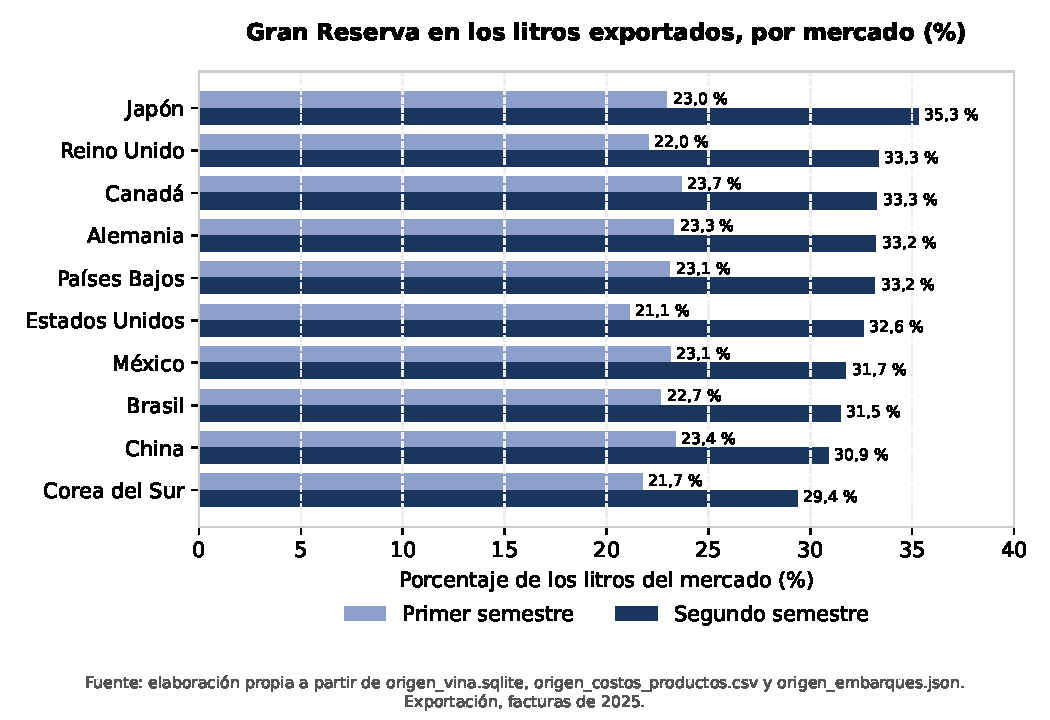
\includegraphics[width=0.58\linewidth]{figura4_gran_reserva_mercados.pdf}
  \caption{Participación de gran reserva en los litros, por mercado y semestre, \%. Fuente: elaboración propia sobre \texttt{fact\_venta}.}
  \label{fig:mercados}
\end{figure}

\noindent La figura respalda el supuesto S8: los diez mercados de exportación suben su participación de gran reserva entre el 1.\textsuperscript{er} y el 2.\textsuperscript{o} semestre, entre 7,5\,pp (China) y 12,3\,pp (Japón). Brasil, el único del hemisferio sur, sube 8,8\,pp.
\clearpage
% Anexo · Declaración de uso de inteligencia artificial.

\section*{Anexo. Declaración de uso de inteligencia artificial}
\label{anexo:ia}
\addcontentsline{toc}{section}{Anexo. Declaración de uso de inteligencia artificial}

Durante el desarrollo de la Entrega~2 y la Presentación~2 se utilizaron herramientas de inteligencia artificial generativa como apoyo técnico y editorial, manteniendo el criterio analítico, las definiciones de negocio y la responsabilidad integral de los resultados en el equipo:

{\sloppy
\begin{itemize}
  \item \textbf{Herramientas utilizadas:} Claude (Anthropic) y Gemini (Google).
  \item \textbf{Propósito de uso:} Refactorización y modularización de los notebooks de la cadena ELT en Databricks (\texttt{src/00\_preparar.py} a \texttt{07\_cifras.py}), estructuración de las pruebas automatizadas de calidad de datos, generación inicial del archivo de definición del tablero (\texttt{vallehondo.lvdash.json}), redacción y edición de secciones en \LaTeX{}, apoyo en la estimación de escenarios de negocio y, con Claude operando el navegador de un integrante, la publicación del tablero y la corrida en un workspace limpio.
  \item \textbf{Verificaciones realizadas a mano por el equipo:}
  \begin{enumerate}
    \item \textbf{Reproducibilidad en ambiente limpio:} La corrida de punta a punta en un workspace independiente de Databricks Free Edition, siguiendo el \texttt{README.md}, la ejecutó Claude en el navegador de un integrante; el equipo revisó el resultado: 8 de 8 pasos, 15 de 15 pruebas en verde y las mismas cifras del informe.
    \item \textbf{Conciliación numérica:} Contraste manual de cada cifra citada en el informe, en la bitácora y en la presentación contra las salidas automatizadas de \texttt{E2/output/cifras.md}, \texttt{cobertura.md} y las vistas en vivo del tablero.
    \item \textbf{Auditoría de consistencia y fuentes:} Revisión línea por línea de las reglas únicas (período, corte, litros por caja y fechas de conversión) en todas las secciones, y cotejo literal de las citas de la contraparte contra las actas y transcripciones del caso.
  \end{enumerate}
\end{itemize}
}

\clearpage
% Anexo · Acta de la reunión del 4 de septiembre (anexo obligatorio del enunciado).
% Se incrusta el PDF que se envió a la contraparte, sin modificar.
% Requiere pdfpages en el preámbulo.

\section*{Anexo. Acta de la reunión del 4 de septiembre}
\addcontentsline{toc}{section}{Anexo. Acta de la reunión del 4 de septiembre}

\noindent Enviada a la contraparte y al cuerpo docente el 8 de septiembre de 2026, dentro del plazo de 48 horas. Se reproduce sin modificaciones.

\medskip
\noindent\textbf{Nota de corrección (noviembre de 2026).} El acta afirma que la unidad de medida de la empresa es el litro. Es una lectura incorrecta de la reunión: operaciones mide en litros, mientras finanzas y comercial venden y hablan en cajas, y la contraparte reconoció no tener gobierno de datos sobre esa equivalencia (V). El texto enviado se conserva sin cambios; la corrección está en la sección~\ref{sec:mandato}.

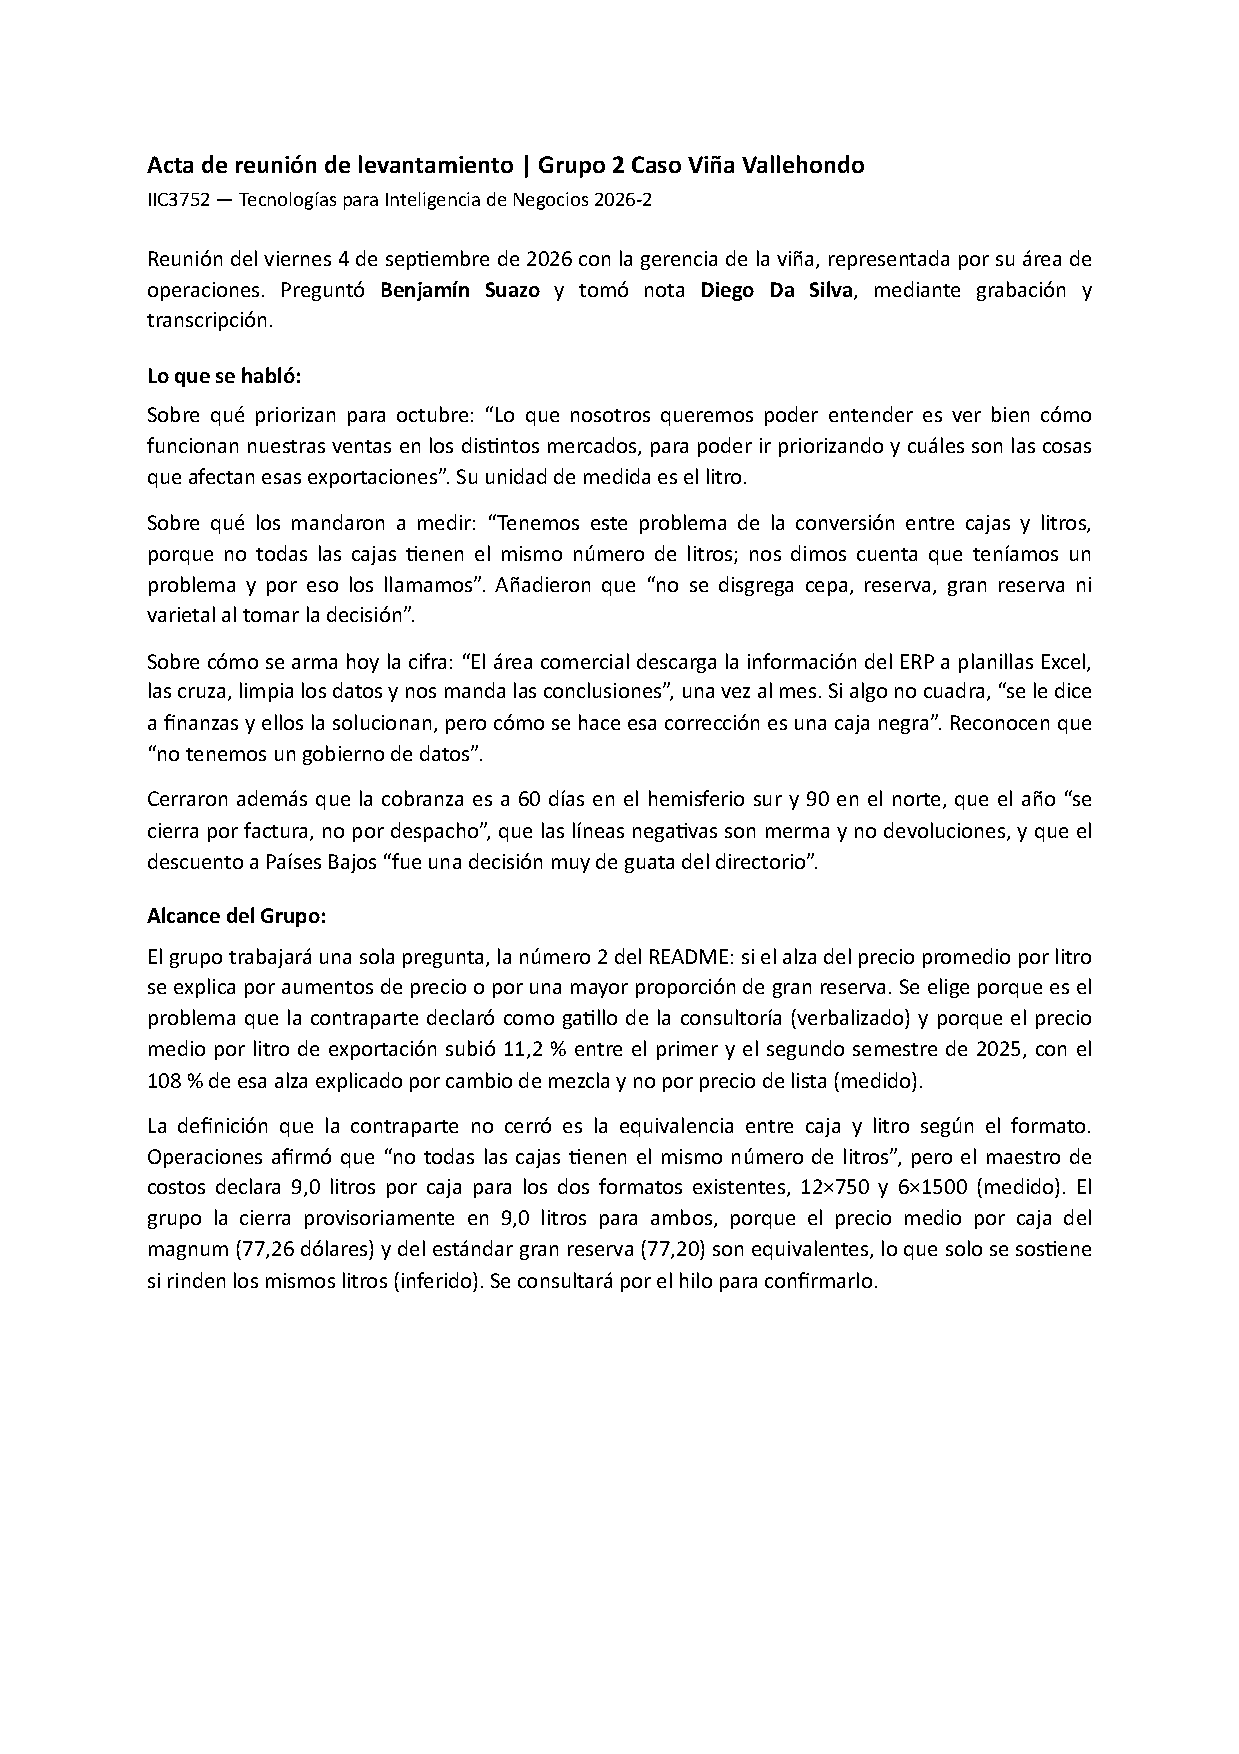
\includepdf[pages=-,scale=0.92]{anexos/Acta_Reunion_Vallehondo_G2.pdf}


\end{document}
